\section{Large Language Models}

When we talk about Large Language Models (LLMs), we refer to advanced software designed to communicate in a human-like manner. These models possess the remarkable ability to understand complex contexts and generate consistent, human-like content. If you have ever interacted with a chatbot or AI virtual assistant, you may have used an LLM without realizing it. LLMs are used in various applications such as text generation, machine translation, sentiment analysis and document summarization, among others. They have become an essential part of the artificial intelligence (AI) landscape. This section delves into their history and evolution, including an analysis of the architecture of the transformer.

LLMs refer to large, general-purpose language processing models that are pre-trained on large datasets to learn the fundamental structures and semantics of human language. The term “large” indicates both the significant amount of data needed for training and the billions or even trillions of parameters these models contain. Pre-training enables LLMs to handle common language tasks such as text classification, question answering and document summarization. After pre-training, these models are typically fine-tuned to smaller, specialized datasets for specific domains, improving their accuracy and efficiency. \cite{researchgraph2024}

\subsection{Evolution of Large Language Models}

\subsubsection{Early Days: Chatbots and Rule-Based Systems (1960s)}

The journey of LLMs began in the 1960s with ELIZA, an early natural language processing computer program created by Joseph Weizenbaum \cite{weizenbaum1966eliza}. ELIZA was able to simulate a conversation by searching for key words and using programmed responses. Following ELIZA, SHRDLU, developed by Terry Winograd in the early 1970s \cite{winograd1972understanding}, was an advanced program capable of understanding and manipulating a virtual block world through natural language commands. This marked a significant step toward machine understanding of context and intentions.

\begin{figure}[h!]
    \centering
    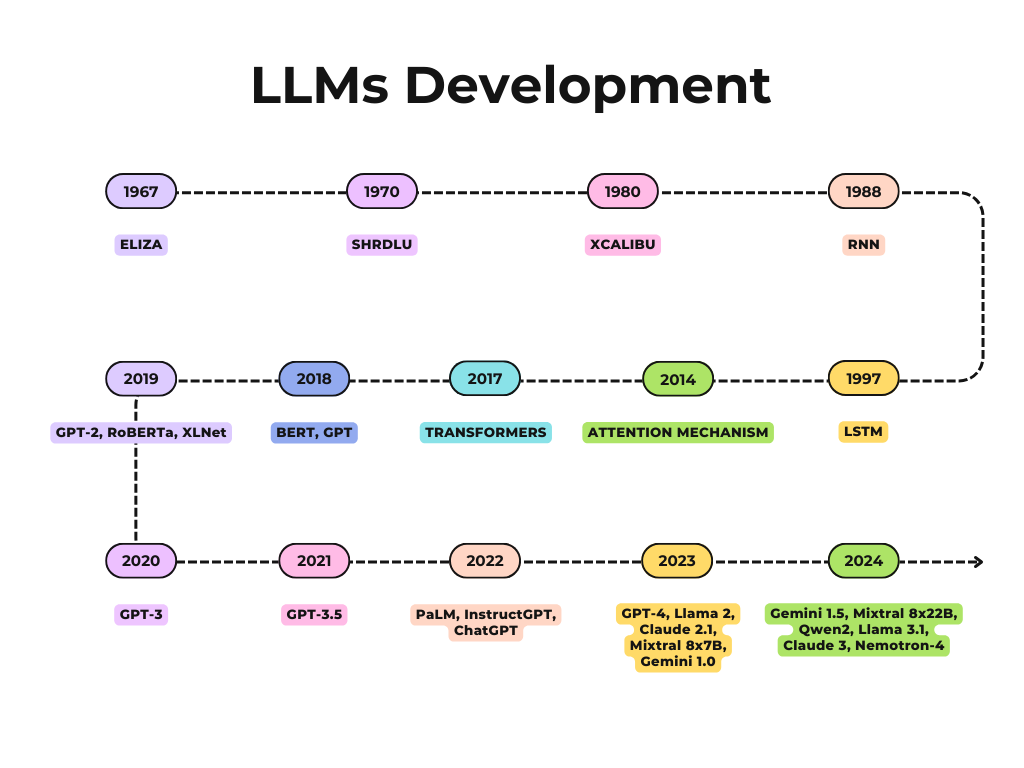
\includegraphics[width=0.8\textwidth]{images/llms/llms-timeline.png}
    \caption{Timeline of Large Language Models (LLMs) development.}
    \label{fig:llms-history}
\end{figure}

\subsubsection{Rise of Recurrent Neural Networks (1980s)}

In the late 20th century, recurrent neural networks (RNNs), inspired by the interconnected neurons of the human brain, were born. Introduced in 1986, RNNs gained popularity for their ability to remember previous inputs and process sequential data, making them suitable for NLP tasks. However, RNNs have had limitations with long sentences, often suffering from the gradient vanishing problem \cite{elman1990finding}.

\subsubsection{Rise of Long Short-Term Memory (1990s)}

Long short-term memory (LSTM), a specialized type of RNNs, was introduced in 1997 to address the limitations of RNNs. LSTMs are capable of remembering information over long sequences, overcoming the short-term memory limitations of RNNs. Their unique architecture, with input, forgetting, and output gates, allowed LSTMs to retain relevant information in memory, making them more efficient for capturing long-term dependencies in sentences \cite{hochreiter1997long}.

\subsubsection{Gated Recurrent Units (2010s)}

In 2014, Gated Recurrent Units (GRUs) were introduced to solve problems similar to LSTMs, but with a simpler structure. GRUs use only two ports: an update port and a reset port, making them more computationally efficient, while maintaining the long-term dependencies in the sentences \cite{cho2014learning}.

\subsubsection{Rise of Attention Mechanism (2014)}

The introduction of the attention mechanism on paper on neural machine translation \cite{bahdanau2014neural} in 2014 marked a paradigm shift in sequence modeling. Unlike RNNs, which process sentences with a context vector of fixed size, attention mechanisms allowed models to dynamically select relevant parts of the source sequence, ensuring that crucial information was not lost, especially in longer sequences.

\subsubsection{The Invention of Transformers Architecture (2017)}

Transformers, introduced in 2017 by Vaswani et al. in the paper “Attention is All You Need” \cite{vaswani2017attention}, relied on an attention mechanism to process sequences. The processors featured an encoder-decoder architecture with multiple layers of self-attention and feed-forward neural networks. The multi-layered attention mechanism allowed the processors to simultaneously focus on different parts of the input sentence, capturing various contextual nuances. Processors could also process sequences in parallel, rather than sequentially, leading to the development of sophisticated LLMs such as BERT and GPT. Given its importance and influence in the AI field, the transformer architecture will be discussed in more depth in later sections.

\subsubsection{Emergence of Large Language Models (2018-Onwards)}

With the success of transformers, scaling these models became the next logical step. Google's BERT model, released in 2018, processed text bidirectionally, setting new performance standards in various benchmarks \cite{devlin2018bert}. OpenAI's GPT-2, released in 2019, and GPT-3 in 2020, demonstrated the capabilities of generative models in performing a wide range of tasks \cite{radford2019language}. OpenAI continued to advance the GPT series with GPT-3.5 in 2022, GPT-4 in 2023 and GPT-4o in 2024. ChatGPT, based on GPT-3.5, became the fastest growing consumer application in history after its release in November 2022.

Other major players in the technology industry and academia have also contributed to the development of LLMs. Google's PaLM (Pathways Language Model) was released in March 2023, followed by PaLM 2 in May 2023 \cite{chowdhery2023palm}. In December 2023, Google unveiled Gemini, a multimodal model capable of processing different forms of information. Meta AI released the LLaMA (Large Language Model Meta AI) series in 2023, offering open-source models for research and commercial use \cite{touvron2023llama}. Anthropic introduced the Claude series in 2023, prioritizing the universal benefits and security of AI \cite{anthropic2024claude}. \newline

The evolution of language models from simple rule-based systems to complex intelligence models means significant progress in artificial intelligence technology. Today, LLMs are more than just tools for improving text-based applications; they are increasingly capable of understanding and communicating with humans. Moreover, multimodal LLMs are able to handle not only text, but also images, sounds and videos, integrating various forms of data to comprehensively understand and analyze different contexts. These models are transforming the way we interact with technology, making it more accessible and responsive to human needs. In essence, LLMs are becoming powerful partners for humans, helping us tackle multiple tasks and simplifying our lives in various ways. \cite{researchgraph2024}

\section{Transformer Architecture}

As mentioned in the previous section, a key breakthrough in language modeling, central to all modern state-of-the-art LLMs, was the introduction of transform architecture and the self-attention mechanism in 2017. This advance was presented in the seminal paper “Attention is All You Need” by Vaswani et al. \cite{vaswani2017attention}, which revolutionized natural language processing (NLP) field by enabling models to capture long-range dependencies much more efficiently than previous architectures.

\begin{figure}[h!]
    \centering
    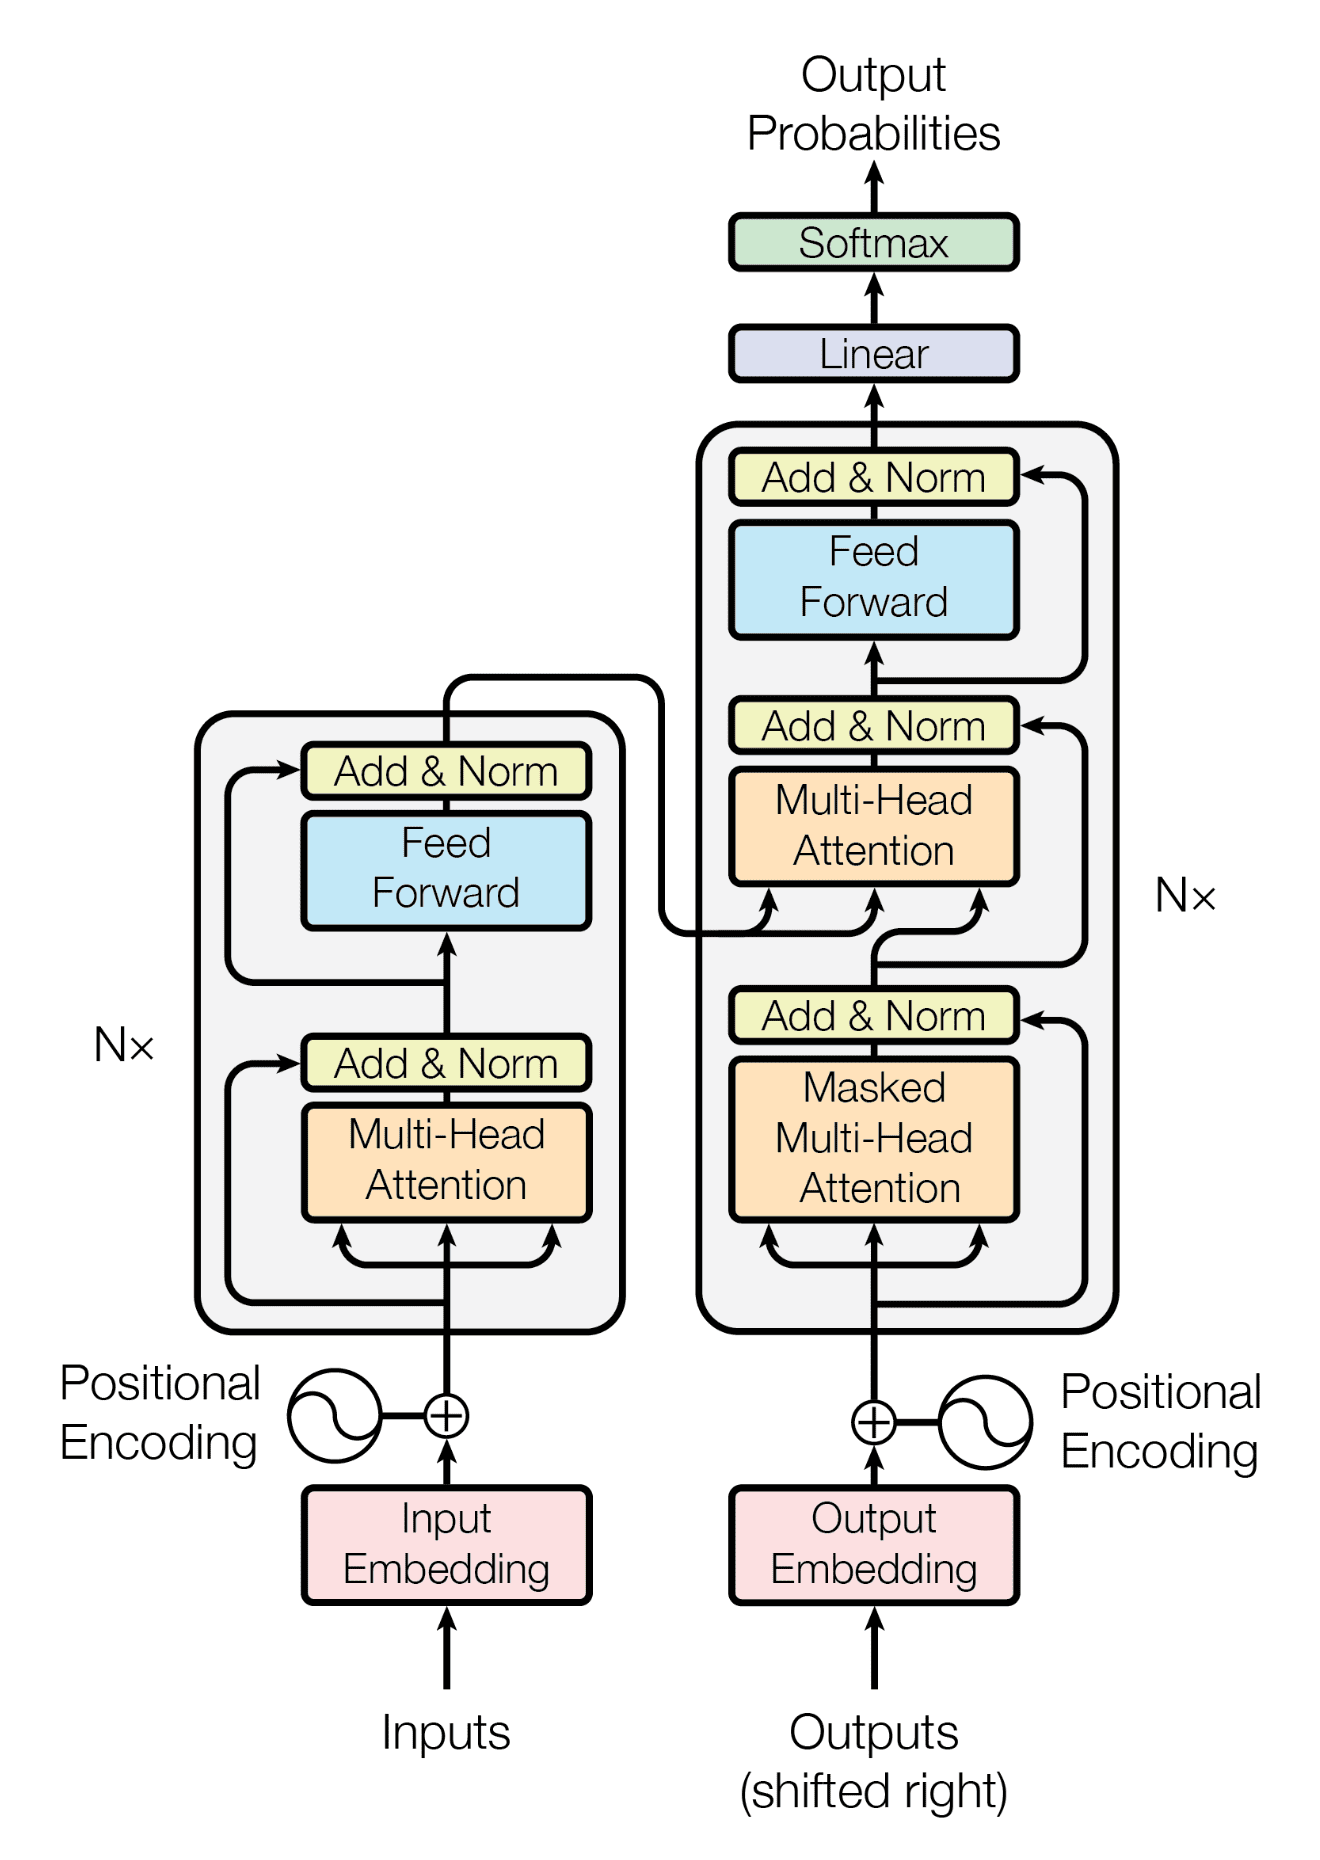
\includegraphics[width=0.6\textwidth]{images/llms/transformer-architecture.png}
    \caption{The general architecture of the transformer, composed of an encoder and a decoder. The encoder takes the input sequence and converts it into continuous representations, while the decoder generates the output sequence from these representations. \textit{Source:} \cite{vaswani2017attention}}
    \label{fig:transformer-architecture}
\end{figure}

The self-attention mechanism is a key component of the transformer, enabling models to weigh the importance of different elements in a sequence by measuring the similarity between elements and determining the amount of attention each element should pay to the others. This mechanism enables the model to grasp complex relationships and dependencies in the entire input sequence, enhancing its ability to understand and generate coherent, context-aware outputs. In NLP, the self-attention mechanism effectively models the relationships between all words in a sentence, facilitating better understanding and generation of text.

The great advantage of the transformer architecture of being highly parallelizable makes it computationally efficient and able to handle input sequences of varying lengths. The ability to process all elements of a sequence simultaneously, rather than sequentially, significantly reduces training time for large data sets. This parallelism, combined with the effectiveness of the self-attention mechanism, has made the transformer the basis for state-of-the-art models in machine translation, text generation and many other NLP tasks.

As illustrated in Figure \ref{fig:transformer-architecture}, the overall transformer architecture consists of an encoder and a decoder, with each component playing a crucial role in processing and sequence generation. The transformative impact of this architecture continues to drive advances in NLP and AI. The key elements of this architecture, such as positional encoding, multi-headed attention, feed-forward neural networks, norm step addition, residual connections, layer normalization, and linear and softmax final layers, will be discussed in the subsequent sections to provide a more detailed understanding of these components.

\subsection{Positional Encoding}

In the field of natural language processing (NLP), transformer models have radically changed our approach to sequence-sequence tasks. Unlike traditional recurrent neural networks (RNNs) or convolutional neural networks (CNNs), transformers process tokens in parallel and have no intrinsic awareness of token order. Positional encodings are a key technique for incorporating transformer models with an understanding of sequence order, enabling them to effectively process and understand input sequences. \cite{li2023transformer}

Positional encodings play a key role in transformer models for several reasons:

\begin{itemize}
    \item \textbf{Preserve sequence order:} Transformer models handle tokens in parallel and have no intrinsic information about token order. Positional encodings provide this information, allowing the model to distinguish tokens based on their position. This is essential for tasks where word order is important, such as language translation and text generation.
    
    \item \textbf{Maintaining Contextual Information:} In NLP tasks, the meaning of a word often depends on its position within the sentence. For example, the word “cat” in “The cat sat on the carpet” has a different meaning than “The carpet sat on the cat.” Positional encodings help maintain this contextual information, allowing the model to understand the correct meaning based on word order.
    
    \item \textbf{Improving generalization}. By incorporating positional information, transformer models can better generalize between sequences of different lengths. This is especially important for tasks where the length of the input sequence varies, such as summarizing documents or answering questions. Positional encodings allow the model to handle input sequences of different lengths without compromising performance.
    
    \item \textbf{Mitigate symmetry:} Without positional encodings, the self-attention mechanism of transformational models treats tokens symmetrically, which can lead to ambiguous representations. Positional encodings introduce asymmetry, ensuring that tokens in different positions are treated distinctly, thus improving the model's ability to capture long-range dependencies \cite{geeksforgeeks2024-pe}.
\end{itemize}

The original transformer paper by Vaswani et al. \cite{vaswani2017attention} introduced sinusoidal positional encodings. The idea is to produce unique encodings for each position that can be added to token embeddings, allowing the model to distinguish the position of each token in a sequence. For position \( p \) and size \( i \), the positional encoding is calculated as:
\begin{equation}
    PE(p, 2i) = \sin\left(\frac{p}{10000^{2i/d}}\right)
\end{equation}

\begin{equation}
    PE(p, 2i + 1) = \cos\left(\frac{p}{10000^{2i/d}}\right)
\end{equation}

where \( d \) is the dimensionality of embeddings. These sinusoidal functions ensure that positional encodings are unique and can convey position-related information that can be used by attention mechanisms. Each dimension of the positional encoding aligns with a sine or cosine function of different wavelengths, creating a geometric progression from \( 2\pi \) to \( 10000 \times 2\pi \). For any fixed offset \( k \), \( PE(p+k) \) can be expressed as a linear function of \( PE(p) \).

Kazemnejad \cite{kazemnejad2019:pencoding} emphasizes the ability of this encoding scheme to capture positional information in a way that satisfies several important criteria: it must produce a unique encoding for each time-step, maintain consistent distances between time-steps in sentences of different lengths, generalize to longer sentences, and remain deterministic.

In more recent large language models (LLMs), positional encoding often uses learned rather than sinusoidal encodings. In this approach, positional encodings are randomly initialized model parameters learned during training, similar to token encodings. The size of the learned positional encoding vector is related to the maximum sequence length that the model can handle. For example, the BERT model \cite{devlin2018bert} employs a positional encoding size of \( 768 \times 512 \), limiting BERT to a maximum input length of 512 tokens. Although the fixed maximum input length is a disadvantage of learned positional encodings, they can adapt during training, allowing the model to learn positional representations better suited to the training data, unlike static sinusoidal encodings.

\subsection{Self-attention mechanism}

The self-attention mechanism is a key component of the transformer architecture, enabling the model to dynamically evaluate the relative importance of different words in a sequence. Initially introduced in the seminal article “Attention is All You Need” by Vaswani et al. \cite{vaswani2017attention}, self-attention is essential for understanding the context and relationships between words, thus enhancing the model's ability to capture long-range dependencies.

In the self-attention mechanism, each token of an input sequence \( X \) with tokens \( x_1, x_2, \ldots, x_n \) is transformed into three vectors:
\begin{itemize}
    \item \textbf{Query (Q):} It represents the token in question.
    \item \textbf{Key (K):} Represents all tokens against which the query is compared.
    \item \textbf{Value (V):} Contains the information of the tokens.
\end{itemize}

These vectors are derived from the embeddings of the input tokens through learned weight matrices \( W_Q \), \( W_K \) and \( W_V \). The self-attention mechanism involves the following steps for each token:

\begin{enumerate}
    \item \textbf{Calculate attention scores:}. This is done by taking the dot product of the Query vector with the Key vectors of all tokens.
    \begin{equation}
        \text{score}(Q, K) = Q \cdot K^T
    \end{equation}
    
    \item \textbf{Softmax normalization:} The scores are rescaled - usually by dividing them by the square root of the depth of the Key vectors, \( \sqrt{d_k} \) - and passed through a softmax function to obtain the attention weights.
    \begin{equation}
        \text{Attention}(Q, K) = \text{softmax}\left(\frac{Q \cdot K^T}{\sqrt{d_k}} \right)
    \end{equation}
    
    \item \textbf{Calculation of output:} The attention weights are used to make a weighted sum of the Value vectors, giving the contextual representation of the token.
    \begin{equation}
        \text{Output} = \text{Attention}(Q, K) \cdot V
    \end{equation}
\end{enumerate}

This self-attention mechanism allows the model to dynamically weigh the importance of different elements in the sequence, facilitating better understanding and generation of the text. The detailed operation of the self-attention mechanism includes calculating attention scores, applying softmax normalization, and obtaining context-aware representations, thus capturing complex relationships and dependencies in the entire input sequence. \cite{geeksforgeeks2024-sa}

\subsection{Multi-Head Attention}

The multi-head attention mechanism enhances the basic self-attention by enabling the model to capture different aspects of the input data more effectively. Instead of performing self-attention once, the transformer executes it multiple times in parallel. This involves multiple sets of weight matrices, allowing the model to learn different representations of the input data.

In multi-head attention, there are \( h \) sets of weight matrices \( W_Q \), \( W_K \), and \( W_V \). Each head independently performs self-attention and produces an output. These outputs are then concatenated and passed through a linear transformation using a learned weight matrix \( W_O \) to produce the final output of the multi-head attention layer:

\begin{equation}
    \text{MultiHeadOutput} = \text{Concat}(\text{head}_1, \text{head}_2, \ldots, \text{head}_h) \cdot W_O
\end{equation}

The learned weight matrix \( W_O \) is optimized during the training process. For models like GPT-4, these weight matrices and other parameters are learned through optimization on a large corpus of training data.

The primary advantage of multi-head attention is that different heads can focus on different parts or aspects of the input data. For instance, in processing a sentence, one head might focus on the grammatical structure, another on the semantics, and yet another on the tone or sentiment. This parallel attention mechanism allows the model to capture a richer and more diverse set of relationships within the input data, leading to more nuanced and accurate outputs \cite{geeksforgeeks2024-sa}.

\begin{equation}
    \text{MultiHead}(Q, K, V) = \text{Concat}(\text{head}_1, \text{head}_2, \ldots, \text{head}_h)W_O
\end{equation}

The multi-head attention mechanism, along with other components of the transformer architecture, significantly advances the field of NLP, enabling the development of powerful language models capable of performing a wide range of tasks with high accuracy and efficiency.

\subsection{Feed-Forward Neural Networks}

In the transformer architecture, after the multi-headed attention mechanism processes the input, each position in the input sequence passes independently through a feed-forward neural network (FFNN). This network is identical for each position, meaning that the same weights and biases are applied regardless of position in the sequence.

The FFNN within the transformer comprises two linear transformations with a ReLU activation function in between:

\begin{itemize}
    \item \textbf{First linear layer}: The input is first multiplied by a weight matrix \( W_1 \) and then a bias is added \( b_1 \), producing a transformed version of the input.
    \item \textbf{ReLU activation}: The output of the first linear layer is then passed through a ReLU (Rectified Linear Unit) activation function. The ReLU function is defined as follows:
    \begin{equation}
        \text{ReLU}(x) = \max(0, x)
    \end{equation}
    This introduces nonlinearity into the model, allowing it to capture more complex patterns in the data.
    \item \textbf{Second linear layer}: The activated output is then passed through another linear layer, multiplying it with a weight matrix \( W_2 \) and adding a bias \( b_2 \). This produces the final output of the FFNN.
\end{itemize}

Given an input \( x \), the FFNN can be represented as:
\begin{equation}
    \text{FFN}(x) = \text{ReLU}(x \cdot W_1 + b_1) \cdot W_2 + b_2
\end{equation}

Where:
\begin{itemize}
    \item \( x \) is the input of the FFNN.
    \item \( W_1 \) and \item \( W_2 \) are weight matrices.
    \item \( b_1 \) and \item \( b_2 \) are bias vectors.
\end{itemize}

All parameters \( W_1 \), \( W_2 \), \( b_1 \) and \( b_2 \) are learnable parameters, optimized during (pre)training.

While the multi-headed attention mechanism allows the model to focus on different parts of the input sequence, FFNN further transforms the attention output. It can be considered an additional level of data abstraction or transformation. The combination of attention and feed-forward mechanisms allows the transformer model to handle a wide range of sequence transduction tasks, such as text synthesis, named entity recognition, or question answering.

\cite{pires2023one} provides an in-depth analysis of the role of FFNNs in transformational models. The authors found that although FFNNs consume a significant portion of the model parameters, they exhibit a significant degree of redundancy. By sharing a single FFNN on all layers of the encoder and removing the FFNN from the decoder, the model achieves substantial parameter savings and faster inference speed, with only a slight decrease in accuracy. The study also explores increasing the amplitude of the shared FFNN, which leads to significant improvements in both accuracy and latency, highlighting the potential for optimizing the use of FFNN in transformer models.

\subsection{Stabilizing Transformer Layers: Add \& Norm Step}

After the multi-headed attention mechanism and feed-forward neural network layer process the inputs in the transformer architecture, the output is stabilized using the add \& norm step. This step is crucial for maintaining model stability and efficiency during training, enabling the architecture to support the deep, multilayer structures common in advanced models. The add \& norm step comprises two main components: the residual connection and layer normalization.

\subsubsection{Residual Connections for Stability (Add)}

Residual connection (or “skip”) provides a shortcut, allowing a sublayer's input to be added directly to its output. This allows the network to effectively learn identity functions; if the best action for a particular layer is to leave the input unchanged, the residual connection layer facilitates this. The weights of the sublayer can be reduced almost to zero, making its output negligible, therefore \(\text{SubLayer}(X) \approx 0\). Adding this data to the original input \(X\) through the residual connection yields an output close to \(X\), resulting in an identity mapping. This mechanism not only increases the performance of the model, but also improves the stability of training. Mathematically, it is represented as:

\begin{equation}
    Z = X + \text{SubLayer}(X)
\end{equation}

Where:
\begin{itemize}
    \item \(X\) is the input to the sublayer.
    \item \(\text{SubLayer}(X)\) signifies the transformations applied by the sublayer to the input \(X\).
    \item \(Z\) is the final output after the residual connection.
\end{itemize}

Residual connections are critical in mitigating the vanishing gradient problem. In deep neural networks with many layers, gradients can decrease during backpropagate, causing the first layers to receive minimal gradient updates, slowing learning or stopping it altogether. Residual connections allow gradients to flow directly through the addition operation without decreasing, ensuring that deep layers also receive substantial gradient updates and solving the vanishing gradient problem.

\subsubsection{Layer Normalization for Consistency (Norm)}

After residual connection, the transformer applies layer normalization to standardize the activations of each feature that has passed through the multi-headed attention layers and FFNNs. This normalization, based on the calculated mean and variance of the activations, scales them so that they have a mean of zero and a standard deviation of one. This normalization ensures that the scale of the activations is consistent, regardless of the layer or input into the transformer.

Given \( Z \) as the input to layer normalization, the mean \( \mu_Z \) and variance \( \sigma_Z^2 \) are computed as:
\begin{equation}
\mu_Z = \frac{1}{d} \sum_{i=1}^{d} Z_i \quad \text{and} \quad \sigma_Z^2 = \frac{1}{d} \sum_{i=1}^{d} (Z_i - \mu_Z)^2
\end{equation}
where \( d \) denotes the feature dimension of \( Z \). Subsequently, the normalized output \( \hat{Z} \) for each feature is calculated as:
\begin{equation}
\hat{Z}_i = \frac{Z_i - \mu_Z}{\sqrt{\sigma_Z^2 + \epsilon}}
\end{equation}

Here, \( \epsilon \) is a small constant added for numerical stability. After normalization, the activations are scaled and shifted using learnable parameters:
\begin{equation}
\text{Norm}(Z)_i = \gamma \hat{Z}_i + \beta
\end{equation}

where \( \gamma \) and \( \beta \) are learnable scaling and shifting parameters, respectively, with the same dimensionality as \( Z \).

Maintaining the activations at a consistent scale across different layers, layer normalization ensures that gradients do not diminish exponentially as they backpropagate through many layers. Consequently, both residual connections and layer normalization address the vanishing (or exploding) gradient problem, enabling the effective training of deep transformer models.

\subsection{Encoder and Decoder Stacks}

The transformer architecture used in state-of-the-art LLMs like GPT-4 \cite{achiam2023gpt} and LLaMA 2 \cite{touvron2023llama} models consists of stacks of encoder and/or decoder blocks. Each block contains multi-head attention and feedforward neural network layers. The stacking of multiple such blocks allows for increased representational power, enabling the model to learn complex patterns and relationships within the data.

The transformer encoder processes the input sequence and transforms it into a series of continuous representations. Each layer of the encoder has a multi-headed self-attention mechanism followed by a fully connected position-based feed-forward network. This design allows the encoder to effectively capture and understand various aspects of the input sequence.

In contrast, the decoder produces the output sequence from the continuous representations provided by the encoder. Similar to the encoder, each layer of the decoder contains a multi-headed self-attention mechanism and a feed-forward network. In addition, the decoder incorporates an attention mechanism between encoder and decoder, which allows it to focus on relevant parts of the input sequence during output generation. This attention mechanism ensures that the output sequence remains contextually consistent with the input sequence.

\subsection{Final Linear and Softmax Layer}

The decoder output goes through a final linear layer and then a softmax layer to create a probability distribution over the target vocabulary. In the context of an NLP task using a transformer model, the target vocabulary includes all possible words, tokens or symbols that the model can generate \cite{jozefowicz2016exploring}. The linear layer converts the high-dimensional representations produced by the decoding stack to a dimensionality that corresponds to the size of the target vocabulary. Next, the softmax function is applied to these raw scores, converting them into probabilities such that the total probability of all vocabulary tokens is equal to one. The resulting probability distribution reflects the model's prediction of the probability that each target vocabulary token is the next token in the sequence, thus enabling operations such as translation and text generation.

\section{Impact of Model Size on AI Performance}

The size of a neural network model, especially in the field of artificial intelligence and natural language processing, is a determining factor in its performance and capabilities. Model size, typically quantified by the number of parameters, affects the model's ability to learn and represent complex data models. Larger models can encapsulate more detailed relationships, resulting in increased accuracy and robustness in various tasks. However, increasing model size also brings challenges, such as increased computational demands, increased memory usage and longer training times.

\subsection{Evolution of Parameter Sizes in AI Neural Networks}

The development of AI neural networks over the years has been characterized by an increase in the number of parameters. In the early days of artificial intelligence, models such as simple feed-forward neural networks and early convolutional neural networks (CNNs) had a relatively modest number of parameters. In fact, before the 2000s, language models were relatively simple and small due to computational limitations. For example, LeNet-5, an early CNN developed by LeCun et al. \cite{lecun1998gradient} in 1998, had about 60,000 parameters. 

As computational capabilities and data availability improved, researchers were able to create larger and more complex models. In particular, the advent of deep learning and the hardware advances of the 2010s led to the emergence of deeper architectures, such as VGGNet and ResNet, which significantly increased parameter sizes. VGG-16, for example, has about 138 million parameters \cite{simonyan2014very}, while ResNet-50 has about 25 million parameters \cite{he2016deep}.

The shift toward larger models has continued with the introduction of transformers and large language models. BERT, introduced by Devlin et al. \cite{devlin2018bert} in 2018, has 110 million parameters in its basic version and 340 million in the larger version. OpenAI's GPT-3 (2020), with 175 billion parameters \cite{brown2020language}, and GPT-4 (2023) with 1.76 trillion parameters \cite{achiam2023gpt} have demonstrated rapid growth in the size of LLM models, establishing new benchmarks in various NLP tasks.

The number of parameters in LLM models significantly affects their ability to capture complex, high-dimensional relationships in data. In general, increasing the number of parameters increases the complexity of the model, which often results in improved performance in various NLP tasks. However, larger models also tend to be more prone to overfitting and require significant computational resources \cite{zhao2023survey, villalobos2022machine, wei2022emergent}.

In addition, the number of parameters of LLMs is related to the volume of their training datasets. Complex models require large and diverse texts to effectively capture the intricate nuances of language. The size of these training datasets is typically measured in tokens, the basic units that LLMs use for text processing and generation. Depending on the tokenization algorithm employed, the tokens may represent individual characters, syllables, words or segments of sentences \cite{brown2020language}.

\subsection{Recent Trends in AI development}

The importance of model size has been further emphasized by recent trends in the development of artificial intelligence, where training computation has emerged as a critical factor. Models with a training computation greater than 10 floating-point operations (FLOP) are depicted in Figure \ref{fig:large-scale-models}. This threshold defines models as "large-scale models," which typically involve training costs of hundreds of thousands of dollars or more. For example, AI Index estimates that OpenAI's GPT-4 used about \$78 million in computation for training, while Google's Gemini Ultra cost \$191 million in computation. \cite{epoch2024trackinglargescaleaimodels,maslej2024ai} 

\begin{figure}[h!]
    \centering
    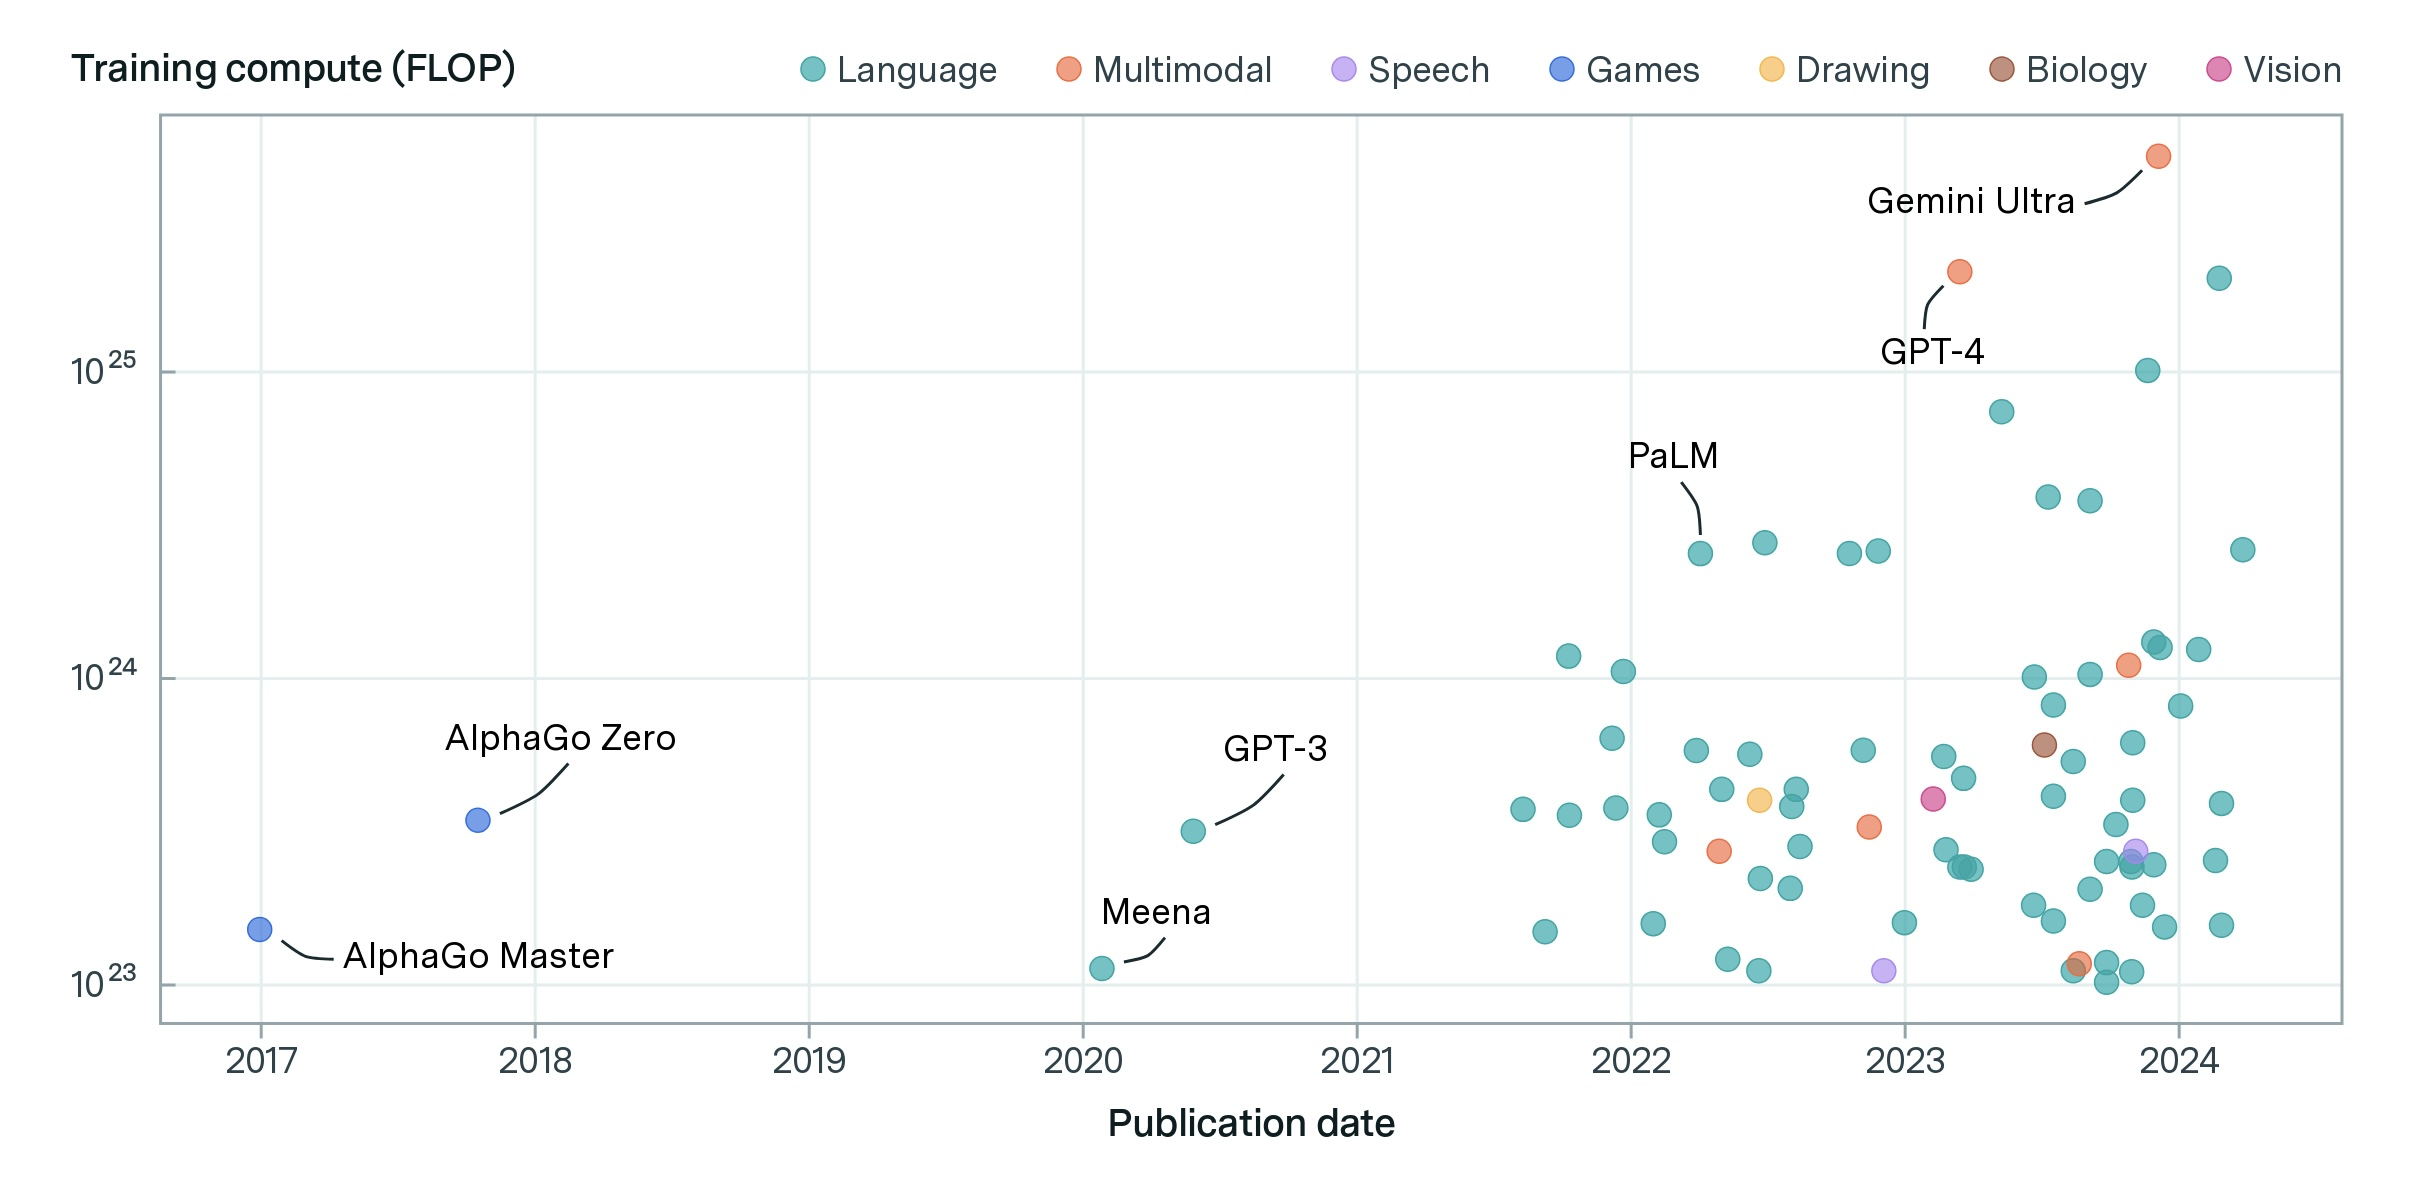
\includegraphics[width=0.9\textwidth]{images/llms/large-scale-models-by-domain-and-date.png}
    \caption{Large-scale models by domain and publication date. The graph displays the training calculation (in FLOP) of various models in different domains over time. \textit{Source:} \cite{epoch2024trackinglargescaleaimodels}}
    \label{fig:large-scale-models}
\end{figure}

In 2020, only 11 models were trained that exceeded the 10\textsuperscript{23} FLOP, but by 2024 the number had risen to 81, indicating a rapid acceleration in the release of large-scale models. Most of these models are linguistic models, while others are multimodal or image processing models. This trend highlights the predominance of language and image generation tasks in AI development since 2021 \cite{epoch2024trackinglargescaleaimodels}.

The rapid advancement of the computational frontier is driven by the exponential increase in ML R\&D investment and hardware performance. Recent trends indicate a growth rate of 4-5 times per year for remarkable models between 2010 and May 2024. For language models in particular, there has been an overall growth rate of up to 9 times per year, attributed to the industry approaching the frontier of artificial intelligence. The continued increase in training computation further underscores the need for efficient hardware and innovative training techniques to support the growth of large-scale AI models \cite{epoch2024trainingcomputeoffrontieraimodelsgrowsby45xperyear}.

A significant portion of large-scale models have been developed in the United States, but China has also contributed an increasing share. The leading organizations with the most confirmed large-scale models are Google, Meta, DeepMind, Hugging Face, and OpenAI. In addition, developers include several companies, universities, and government institutions. When considering unconfirmed models, organizations such as Anthropic and Alibaba also occupy a prominent position. Most of the large-scale models are produced by industry rather than academia, some are the result of industry-university collaborations, and a couple are developed by government institutions. Notably, almost half of the large-scale models have downloadable and publicly available weights, mainly trained with calculations between 10\textsuperscript{23} and 10\textsuperscript{24}. FLOP. However, larger proprietary models often use much higher computational resources and do not disclose training details.

However, the growth frontier has shown signs of slowing due to potential obstacles such as data scarcity, willingness to invest, data center power restrictions, or the inability to scale chip production. These factors may have an impact on the exponential growth of computing resources required for training advanced AI models \cite{epoch2024trainingcomputeoffrontieraimodelsgrowsby45xperyear}.

In conclusion, model size plays a key role in the performance of AI neural networks. The trend toward larger models has led to significant advances in AI capabilities, especially in the field of NLP. However, it also requires a careful balance between performance and practical considerations, such as computational efficiency and resource demands. The continued increase in training computation and associated challenges highlight the need for innovative approaches to maintain the trajectory of AI progress.

\section{Training Process}

Training large language models (LLMs) is a complex process comprising a series of discrete stages, each of which is designed to enhance the model's capabilities in a gradual and systematic manner. The training of these sophisticated models, which include billions of parameters, has been made possible by recent advances in computing power and architectural innovations. The training process is comprised of three distinct phases: pre-training, fine-tuning, and prompt-based learning. Each phase contributes uniquely to the development and refinement of the model (Figure \ref{fig:training-process}).

Large language models undergo an initial phase of pre-training, during which the model is trained on a substantial unlabeled dataset, which frequently encompasses a significant portion of internet text. This phase enables the LLM to develop a foundational comprehension of language structures and patterns through the recognition and learning from the input data. Following the completion of the pre-training phase, the models are then subjected to a fine-tuning process utilising smaller, task-specific datasets. The objective of this tuning process is to adapt the model's capabilities to perform specialized tasks, such as translation, question answering, or chatbot functionality. Prompting entails engaging with an optimized model through the use of specific questions or statements, referred to as prompts, with the objective of eliciting the desired response from the model. The following sections will examine these three essential elements of LLM training and the methodologies employed to train LLMs for question-answering chatbot applications.


\begin{figure}[h!]
    \centering
    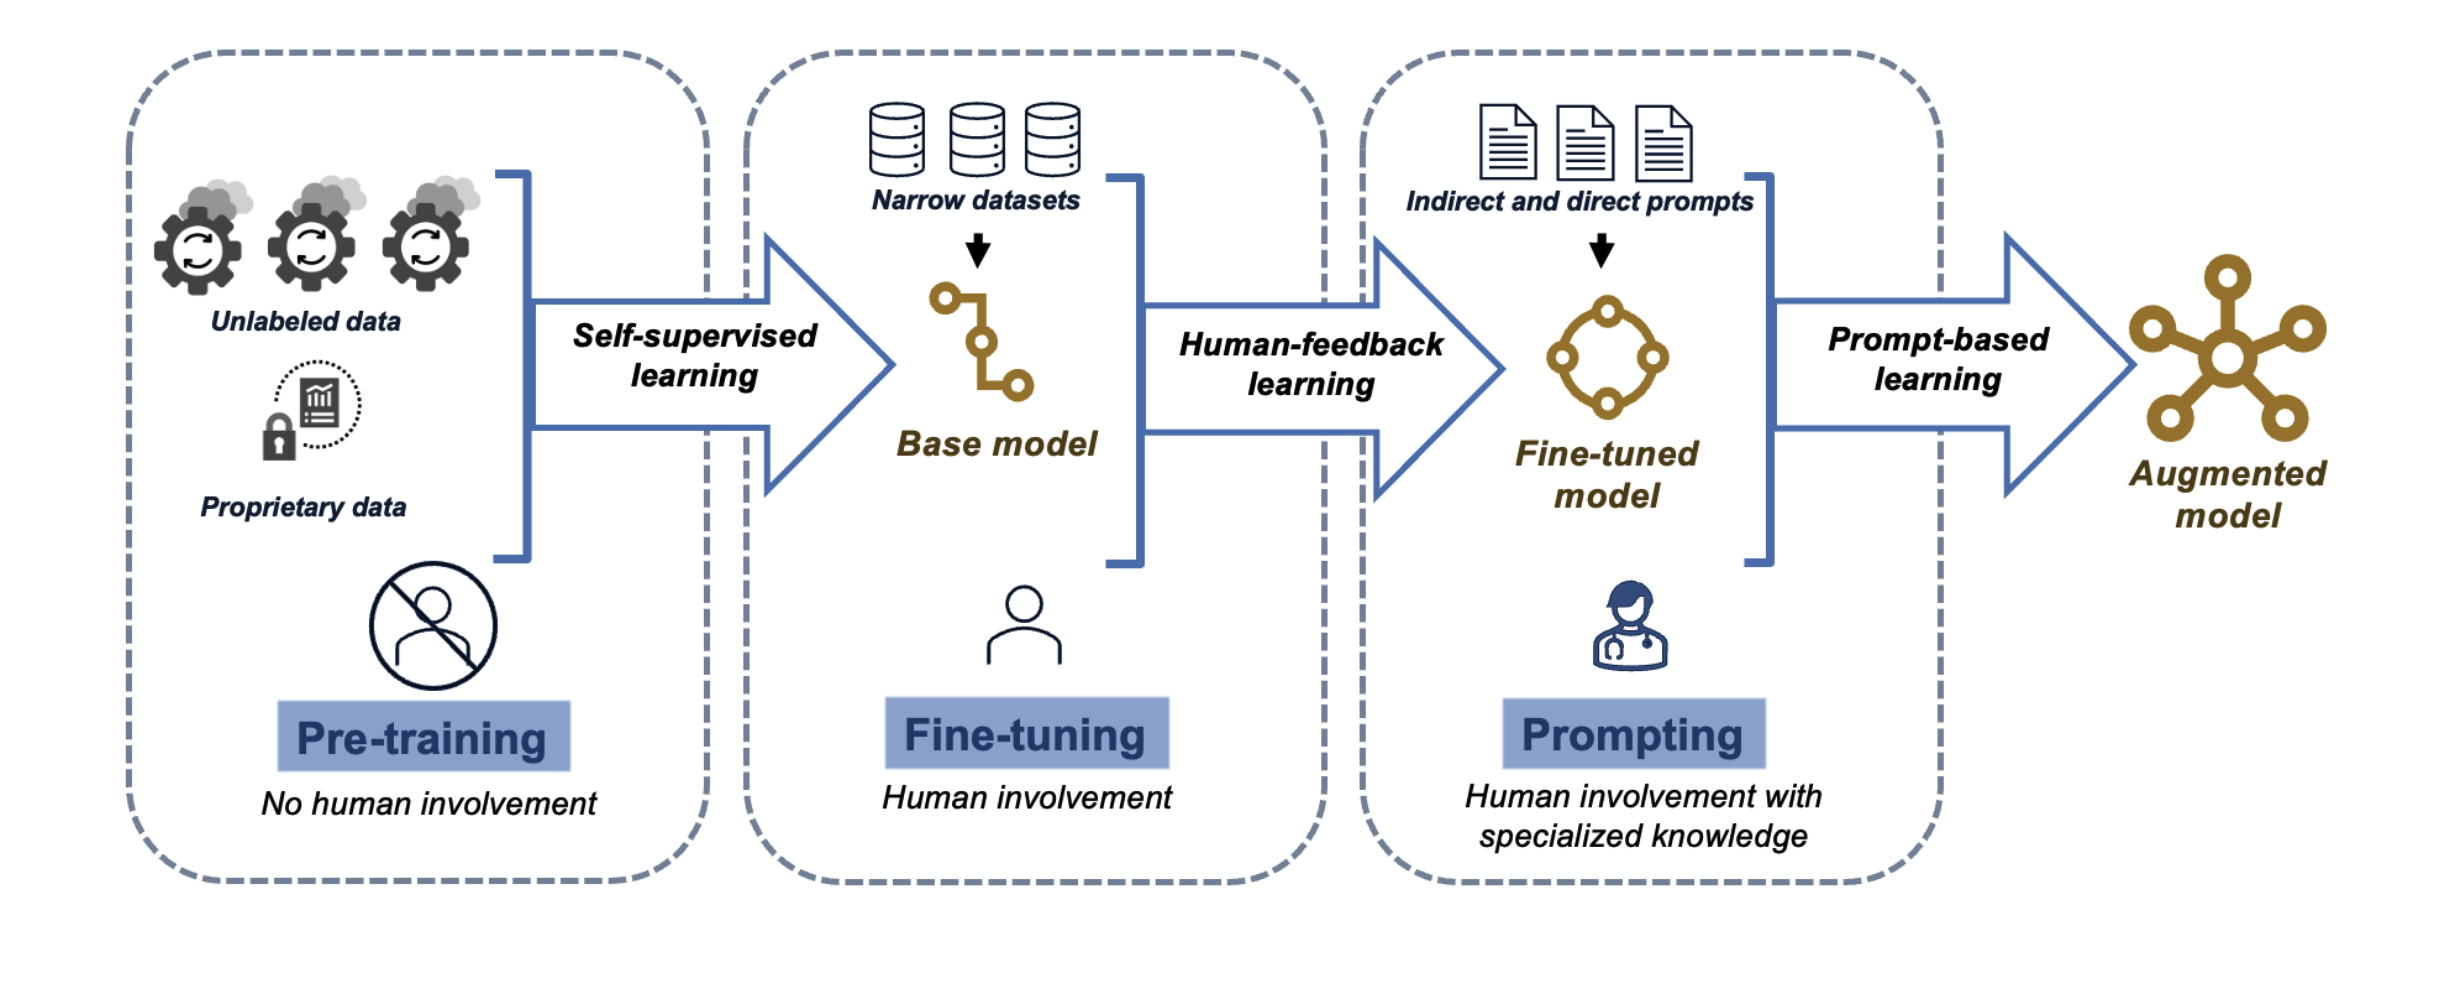
\includegraphics[width=0.9\textwidth]{images/llms/LLM-training-process.png}
    \caption{Overview of the training process of LLMs. LLMs learn from more targeted inputs at each stage of the training process. The first phase of this learning is pre-training, in which the LLM can be trained on a mix of unlabeled data without any human supervision. The second phase is fine-tuning, in which narrower data sets and human feedback are introduced as inputs to the basic model. The fine-tuned model can then enter a further phase, in which humans with specialized knowledge implement hinting techniques that can transform the LLM into an enhanced model to perform specialized tasks. \textit{Source:} \cite{omiye2023large}}
    \label{fig:training-process}
\end{figure}

\subsection{Pre-training}

The pre-training phase is a critical component in the development of LLMs, enabling them to understand and generate human language. This phase is a self-supervised process in which the model is trained on a large corpus of unlabeled data, such as Internet texts, Wikipedia, Github code, social media posts, and BooksCorpus. Some models also incorporate proprietary datasets containing specialized texts such as scientific articles \cite{brown2020language, devlin2018bert}.

The primary objective during the pre-training phase is to predict the subsequent word in a sentence. This is a computationally demanding task that entails converting the text into tokens prior to entering them into the model proposed by Radford et al. \cite{radford2019language}. This phase yields a rudimentary model that, while capable of generating general language, is unable to perform tasks requiring nuance.

The two principal methods for pre-training are Autoregressive Language Modeling (ALM) and Masked Language Modeling (MLM). Both approaches have had a significant impact on the development of state-of-the-art LLMs, enhancing their capacity to comprehend and produce texts that are akin to those produced by humans.

\subsubsection{Autoregressive Language Modeling (ALM)}

In the context of natural language processing, autoregressive language modeling represents a generative approach whereby the model is tasked with predicting the subsequent word in a sequence, given the preceding words. Autoregressive language models, exemplified by GPT (Generative Pre-trained Transformer), have attracted considerable attention due to their remarkable proficiency in generating high-quality text and executing a diverse range of language-related tasks. These models employ a transformer architecture to facilitate the sequential processing of textual data. The autoregressive mechanism enables the generation of coherent and contextually relevant text by sampling from the learned probability distribution over the vocabulary. This has been demonstrated in previous studies, including those by Radford et al. (2018, 2019) and Achiam (2023), which used GPT as a case study \cite{radford2018improving, radford2019language, achiam2023gpt}.

All autoregressive models developed by OpenAI have employed a semi-supervised learning approach, which combines elements of both supervised and unsupervised learning. Specifically, OpenAI introduced a methodology involving unsupervised pre-training followed by supervised fine-tuning, which addresses the high costs associated with the creation of labeled datasets for language tasks.

\begin{figure}[h]
    \centering
    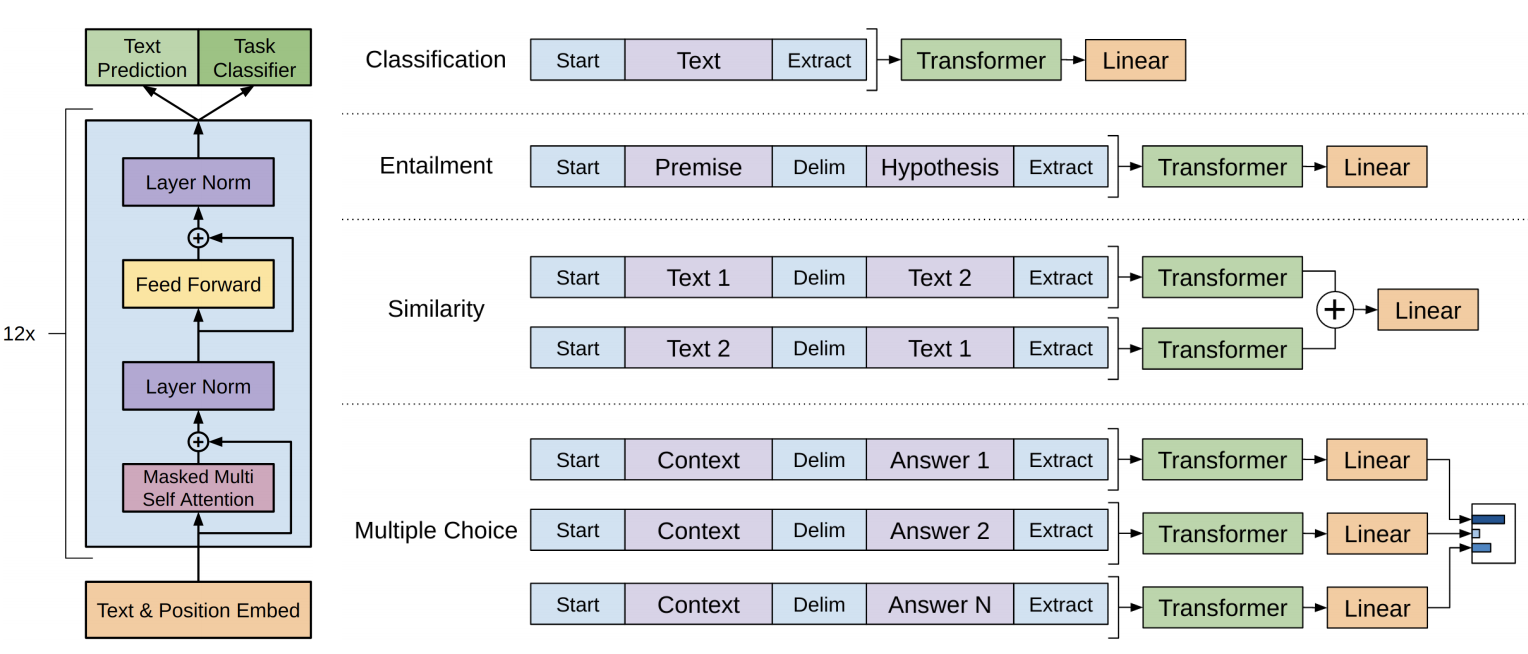
\includegraphics[width=0.9\textwidth]{images/llms/gpt.png}
    \caption{The architecture of the decoder represents the transformer of a GPT, which has been trained for the purpose of auto-regressive text generation. The diagram demonstrates the integration of text prediction and task-specific classifiers, as well as the application of multi-headed self-attention and feed-forward neural networks. \textit{Source:} \cite{radford2018improving}}
    \label{fig:transformer_architecture}
\end{figure}

In unsupervised pre-training, a high-capacity language model is trained on an extensive corpus of text with the objective of maximizing the log-likelihood of the next word given the context provided by the preceding sequence. The formal objective is stated as follows:

\begin{equation}
    \mathcal{L}_1(\mathcal{U}) = \sum_{i} \log P(u_i | u_{i-k}, \ldots, u_{i-1}; \Theta)
\end{equation}

where \( k \) represents the context window. In simpler terms, the model looks back at \( k \) tokens while predicting the \((k+1)^{th}\) token. In the pre-training phase, a multi-layer transformer decoder is utilized. Subsequently, multi-headed self-attention is applied to the input tokens, followed by a position-wise feed-forward network. The resulting output is a distribution over the target tokens.

This is subsequently followed by a supervised fine-tuning phase, where a labeled dataset with \( y \) as labels and \( x \) as inputs is utilized. The inputs are passed through the pre-trained model, and the output from the final transformer block is fed into an additional linear output layer with parameters \( W_y \) to predict \( y \). This process results in the following intermediate objective to maximize:

\begin{equation}
    \mathcal{L}_2(\mathcal{C}) = \sum_{(x,y)} \log P(y | x^1, \ldots, x^m)
\end{equation}

The incorporation of the pre-training objective as an auxiliary objective during fine-tuning has been demonstrated to enhance generalization and accelerate convergence, as evidenced by research findings. Consequently, the pre-training loss \( \mathcal{L}_1 \) is integrated into the final objective with a weighting factor \( \lambda \):

\begin{equation}
    \mathcal{L}_3(\mathcal{C}) = \mathcal{L}_2(\mathcal{C}) + \lambda \ast \mathcal{L}_1(\mathcal{C})
\end{equation}
 
\subsubsection{Masked Language Modeling (MLM)}

Masked Language Modeling, on the other hand, is a denoising goal used primarily by models such as BERT (Bidirectional Encoder Representations from Transformers) \cite{devlin2018bert}. In MLM, certain tokens in the input sequence are randomly masked, and the model is tasked with predicting these masked tokens based on their surrounding context. This bidirectional approach allows the model to understand context from both the left and the right of the masked token, providing a more holistic understanding of the text.

The MLM approach has several advantages. By leveraging bidirectional context, MLM models can develop a comprehensive understanding of language patterns and dependencies. This capability is particularly beneficial for tasks that require nuanced understanding, such as question answering and natural language inference. In addition, the MLM pre-training goal has been shown to enhance the model's generalization capabilities, leading to improved performance in various downstream tasks \cite{yang2019xlnet}.

\begin{figure}[h]
    \centering
    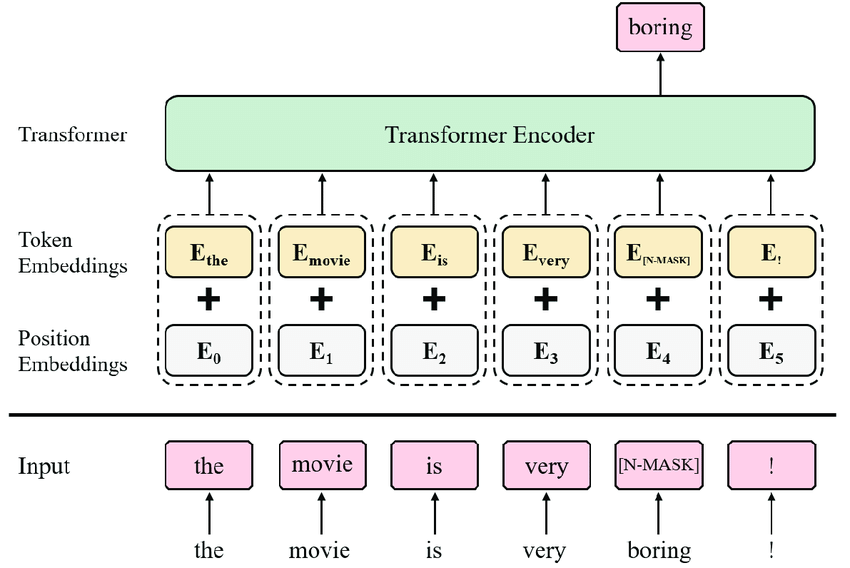
\includegraphics[width=0.8\textwidth]{images/llms/Model-structure-of-the-label-masked-language-model-N-MASK-is-a-mask-token-containing.png}
    \caption{An illustration of Masked Language Modeling (MLM) in a transformer architecture. The input sequence contains masked tokens that the model attempts to predict based on the context provided by the surrounding tokens. Token embeddings are combined with positional embeddings before being fed into the transformer encoder. The final output is a prediction of the masked token using the bidirectional context. \textit{Source:} \cite{park2019}}
    \label{fig:mlm_architecture}
\end{figure}

The introduction of MLM has significantly advanced the field of natural language processing. Models pre-trained with MLM have achieved state-of-the-art results on numerous benchmark datasets, demonstrating their effectiveness in capturing complex linguistic patterns. For example, BERT has set new performance standards on the General Language Understanding Evaluation (GLUE) benchmark \cite{wang2018glue}.

In addition, subsequent variations and extensions of the MLM approach, such as RoBERTa \cite{liu2019roberta} and XLNet \cite{yang2019xlnet}, have further pushed the boundaries of what is possible with pre-trained language models. These models have refined the MLM methodology, incorporating larger training corpora and more sophisticated training strategies to achieve even better results.

\subsubsection{Comparative Analysis}

Compared to Autoregressive Language Modeling (ALM), MLM offers distinct advantages for tasks that require a holistic understanding of context. While ALM generates text sequentially, limiting its context to preceding tokens, MLM's bidirectional nature allows it to consider both preceding and succeeding tokens, providing a richer context for language understanding. However, MLM is not inherently suited to text generation tasks without additional modifications, whereas ALM excels at such generative tasks.

Both ALM and MLM have their strengths and trade-offs. ALM is inherently sequential and excels at text generation tasks where text flow is critical. However, its unidirectional nature can limit its performance in understanding context that spans both directions. On the other hand, MLM's bidirectional context understanding makes it powerful for tasks such as question answering and natural language inference, although it is not directly suited for text generation tasks without additional fine-tuning.

The choice between ALM and MLM during pre-training depends on the intended use of the LLM. In practice, combining these approaches can yield models that leverage the strengths of both, as seen in some recent advances in the field \cite{lewis2019bart}.

Understanding autoregressive and masked language modeling is fundamental to appreciating the design and capabilities of modern LLMs. These methods underpin the pre-training phase and set the stage for the remarkable performance of models in various NLP tasks.

\subsubsection{Next-Token Prediction and Multi-Token Prediction}

Next-token prediction is a fundamental task in training large language models (LLMs), where the model is trained to predict the next word in a sequence given the previous words. Formally, given a sequence of tokens \( \{x_1, x_2, \ldots, x_T\} \), the model learns to estimate the probability distribution \( P(x_t | x_1, x_2, \ldots, x_{t-1}) \). The learning objective is to minimize the cross-entropy loss:

\begin{equation}
    \mathcal{L}_1 = - \sum_{t} \log P_\theta (x_{t+1} | x_1, \ldots, x_t),
\end{equation}

where \( P_\theta \) is our large language model under training, aiming to maximize the probability of \( {x_{t+1}} \) as the next future token, given the history of past tokens \( {x_1, \ldots, x_t} \).

Recently, a novel methodology known as multi-token prediction has been proposed to improve the training efficiency and performance of LLMs. In this approach, the model predicts multiple future tokens simultaneously, rather than one token at a time. This method leverages a shared model trunk and multiple independent output heads to predict the next \( n \) tokens in parallel. This leads to the following factorization of the multi-token prediction cross-entropy
loss:

\begin{equation}
    \mathcal{L}_n = - \sum_{t} \sum_{i=1}^{n} \log P_\theta (x_{t+i} | z_{t:1}) \cdot P_\theta(z_{t:1} | x_{t:1}).
\end{equation}

In practice, as illustrated in Figure \ref{fig:multi-token-prediction}, the model architecture consists of a shared transformer backbone \( f_s \) that produces the hidden representation \( z_{t:1} \) from the observed context \( x_{t:1} \). Additionally, there are \( n \) independent output heads implemented as transformer layers \( f_{h_i} \), along with a shared unembedding matrix \( f_u \). Therefore, to predict \( n \) future tokens, we compute:

\begin{equation}
    P_\theta(x_{t+i} | x_{t:1}) = \text{softmax}(f_u(f_{h_i}(f_s(x_{t:1})))),
\end{equation}

for \( i = 1, \ldots, n \), where specifically \( P_\theta(x_{t+1} | x_{t:1}) \) represents our next-token prediction head.

This multi-token prediction approach has demonstrated significant improvements in sampling efficiency and downstream performance, especially for larger model sizes and for tasks such as code generation. It has been shown that models trained with multi-token prediction can achieve higher accuracy on generative benchmarks such as HumanEval and MBPP, significantly outperforming models trained with traditional next-token prediction. In addition, multi-token prediction enhances the model's ability to perform algorithmic reasoning tasks and improves its out-of-domain generalization capabilities \cite{gloeckle2024better}.

\begin{figure}[h]
    \centering
    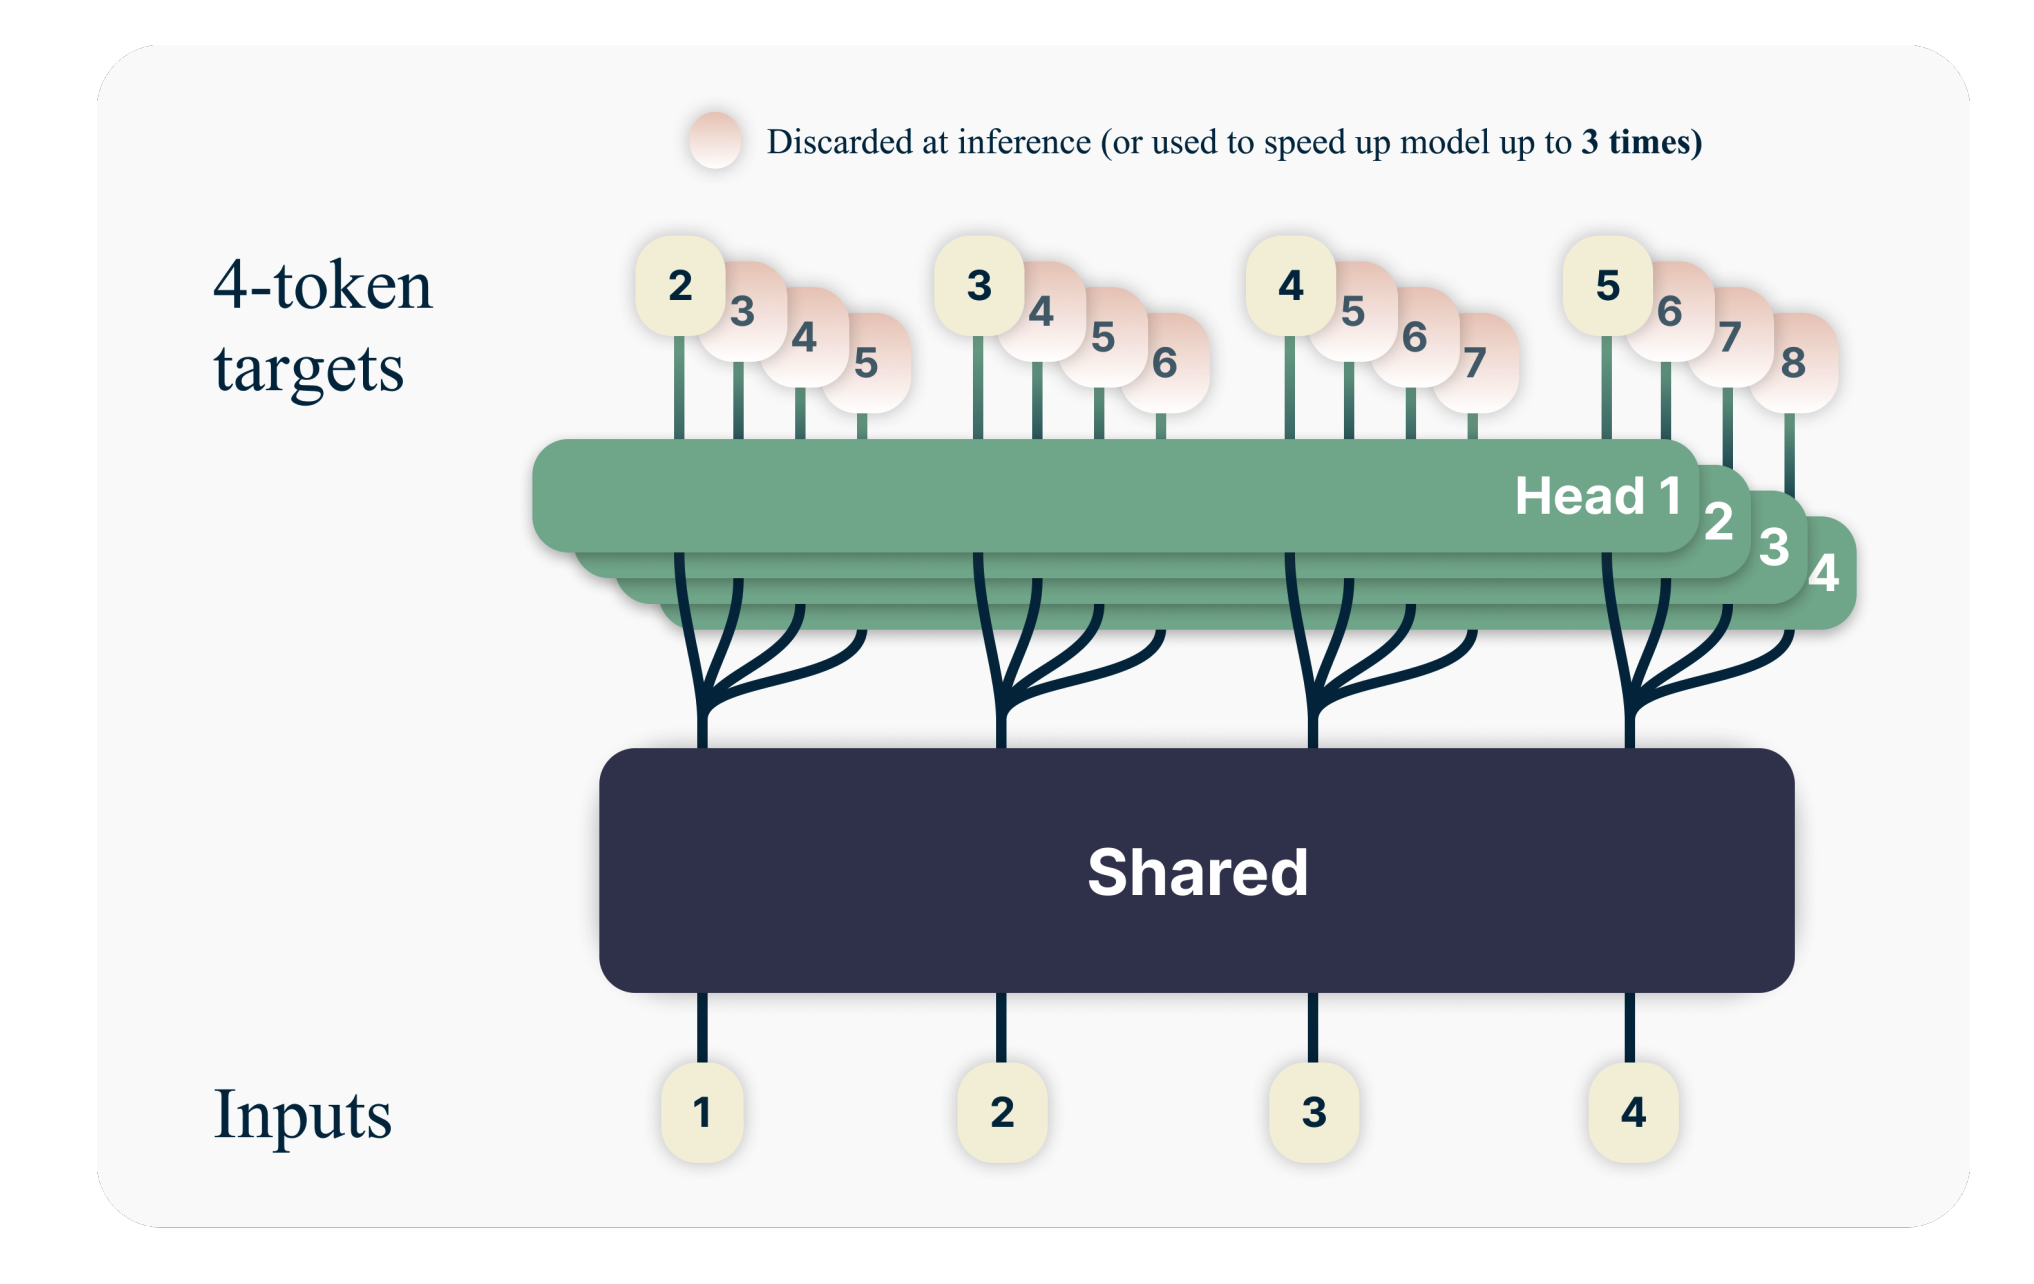
\includegraphics[width=0.8\textwidth]{images/llms/multi-token-pred-architecture.png}
    \caption{Overview of the Multi-Token Prediction Architecture. The model predicts four future tokens simultaneously using a common trunk and four independent output heads. This setup improves sampling efficiency and inference speed. The performance gains are particularly noticeable for larger models and for generative tasks. \textit{Source:} \cite{gloeckle2024better}}
    \label{fig:multi-token-prediction}
\end{figure}

In conclusion, multi-token prediction offers a promising improvement over next-token prediction by allowing models to learn more efficiently and effectively. This methodology not only speeds up the training process, but also improves the overall performance of LLMs in various generative and reasoning tasks.

\subsection{Fine-tuning}
% Introduction of fine-tuning + Differences from Pretraining
% TODO

Following the completion of the pre-training phase, the models are prepared for adaptation to a multitude of downstream tasks. This versatility and broad applicability serve to underscore the foundational yet incomplete nature of these models. For these and other reasons, these models are designated as "foundational".

First, they are pivotal to the advancement of AI, providing the foundation upon which more sophisticated models can be constructed and refined. Their capacity to process a multitude of tasks across diverse domains, including language, vision, robotics, reasoning, and human interaction, illustrates their foundational role in AI research and application.

Secondly, the term "foundation" underscores the pivotal yet nascent status of these models. Despite their impressive capabilities, these models possess emergent properties that are not yet fully understood, and their large scale introduces new, unforeseen abilities. These models are constructed on the tenets of deep learning and transfer learning, yet their efficacy across a multitude of tasks gives rise to a tendency towards homogeneity. While this homogenization offers significant advantages, it also means that any defects or biases present in the foundation models are propagated to all downstream models adapted from them \cite{bommasani2021opportunities}.

This adaptation phase is called fine-tuning and it constitutes a further training of the foundation model on narrower, domain-specific datasets. For instance, models can be fine-tuned on medical transcripts for healthcare applications or on legal briefs for legal assistant bots \cite{radford2019language}. Fine-tuning involves modifying the model’s weights to optimize its performance for the particular nuances and vocabulary of the task-specific data. This process entails adjusting the model's parameters (weights) according to the task-specific data, which often includes labeled examples for supervised tasks.

Fine-tuning can be enhanced through approaches such as Constitutional AI, which embeds predefined rules into the model's architecture, and reward training, where humans evaluate the quality of multiple model outputs \cite{bai2022constitutional}. Furthermore, reinforcement learning from human feedback (RLHF) is employed, which uses a comparison-based system to optimize model responses. While fine-tuning is less computationally intensive, it necessitates substantial human input to adapt the model for particular tasks with predefined outputs. The model that has undergone fine-tuning is then deployed in a variety of applications, including chatbots \cite{ouyang2022training}.

\section{Methods of Fine-Tuning}

	•	Parameter Efficient Fine-Tuning (PEFT)
	•	LoRA (Low-Rank Adaptation)
	•	Adapters
	•	Prefix Tuning

\subsubsection{Full Model Fine-Tuning}

Full model fine-tuning represents the most straightforward approach, whereby all parameters of the pre-trained model are updated during the fine-tuning process. This approach is particularly effective when the target task bears a strong resemblance to the tasks on which the model was originally pre-trained. The advantage of full model fine-tuning is its capacity to adapt the model to the specific nuances of the new task, which may result in enhanced performance \cite{howard2018universal}.

Nevertheless, the increasing size of LLMs over the years has rendered the fine-tuning process extremely computationally demanding and time-consuming. These challenges have significantly increased operational costs, and the financial burden of maintaining and deploying multiple instances of these fine-tuned models becomes especially pronounced when managing numerous downstream tasks.

In light of these challenges, alternative fine-tuning approaches, such as Parameter Efficient Fine-Tuning (PEFT) methods, have been developed with the objective of optimizing the process, thereby reducing the computational and financial burdens associated with full model fine-tuning.

\subsubsection{Layer-wise Fine-Tuning}

Layer-wise fine-tuning represents a more refined approach to model fine-tuning, whereby the model is fine-tuned in stages, starting with the top layers (closer to the output) and gradually incorporating lower layers (closer to the input). This method allows for more precise adaptation, which can be particularly advantageous when the target task necessitates only minor modifications to the pre-trained model. The application of layer-wise fine-tuning can serve to mitigate the issue of overfitting by limiting the extent of alterations made to the model's parameters. This approach is often utilized in scenarios where computational resources are constrained or when dealing with smaller datasets \cite{ro2021autolr}.

\subsubsection{Adapter Layers}

Adapter layers provide a flexible and efficient alternative to full model fine-tuning. In this technique, small neural network modules, referred to as "adapters," are inserted into the layers of the pre-trained model. During the fine-tuning process, only the parameters of the adapter layers are updated, while the original model parameters remain fixed. This approach markedly diminishes the number of parameters that require modification, consequently reducing computational costs and accelerating training times. Adapter layers have been demonstrated to perform at a comparable level to full model fine-tuning, particularly in low-resource settings. Furthermore, they have been shown to be highly effective for multi-task learning, where the same pre-trained model can be fine-tuned for different tasks by simply switching the adapters. \cite{houlsby2019parameter}.

\subsection{Parameter Efficient Fine-Tuning (PEFT)}

In order to address the considerable computational and financial costs associated with the vast scale of LLM systems, the parameter-efficient fine-tuning (PEFT) approach was developed as a viable solution to this challenge. This approach facilitates the efficient adaptation of large models to a range of downstream tasks, thereby reducing the burden of significant costs. PEFT entails the process of fine-tuning a pre-trained large model to a specific task or domain while minimizing the number of additional parameters introduced and the computational resources required \cite{han2024parameter}.

Among the various PEFT techniques, Low-Rank Adaptation (LoRA) is distinguished by its efficacy in reducing the computational demands associated with fine-tuning large-scale models. For this reason, LoRA will be introduced in the following section.

\subsection{LoRA: Low-Rank Adaptation}

To address the increasing scale of models, Low-Rank Adaptation (LoRA) has been proposed. This method involves freezing the pre-trained model weights and incorporating trainable rank decomposition matrices into each layer of the Transformer architecture. This significantly reduces the number of trainable parameters required for downstream tasks. In comparison to fine-tuning GPT-3 175B using Adam, LoRA achieves a reduction in trainable parameters by a factor of 10,000 and decreases the GPU memory requirement by a factor of three.

Unlike traditional fine-tuning, which necessitates adjusting the entire model, LoRA focuses on modifying a smaller subset of parameters (lower-rank matrices), thereby reducing computational and memory overhead. This approach is predicated on the understanding that large models inherently possess a low-dimensional structure. By leveraging low-rank matrices, LoRA effectively adapts these models, allowing significant model changes to be represented with fewer parameters, thereby optimizing the adaptation process \cite{hu2021lora}.

\subsubsection{Decomposition in LoRA}

In traditional fine-tuning the weights of a pre-trained neural network are modified to adapt to a new task. This adjustment involves altering the original weight matrix \( W \) of the network. The changes made to \( W \) during fine-tuning are collectively represented by \( \Delta W \), such that the updated weights can be expressed as \( W + \Delta W \).

Rather than modifying \( W \) directly, the LoRA approach decomposes \( \Delta W \). This decomposition is crucial in reducing the computational overhead associated with fine-tuning large models.

The intrinsic rank hypothesis suggests that significant changes to the neural network can be captured using a lower-dimensional representation. Essentially, it posits that not all elements of \( \Delta W \) are equally important; instead, a smaller subset of these changes can effectively encapsulate the necessary adjustments.

Building on this hypothesis, LoRA represents \( \Delta W \) as the product of two smaller matrices, \( A \) and \( B \), with a lower rank. The updated weight matrix \( W' \) thus becomes:

\begin{equation}
    W' = W + BA
\end{equation}

In this equation, the variable \( W \) is held constant, indicating that it is not updated during the training process. The matrices \( B \) and \( A \) are of lower dimensionality, with their product \( BA \) representing a low-rank approximation of \( \Delta W \).

\begin{figure}[h]
    \centering
    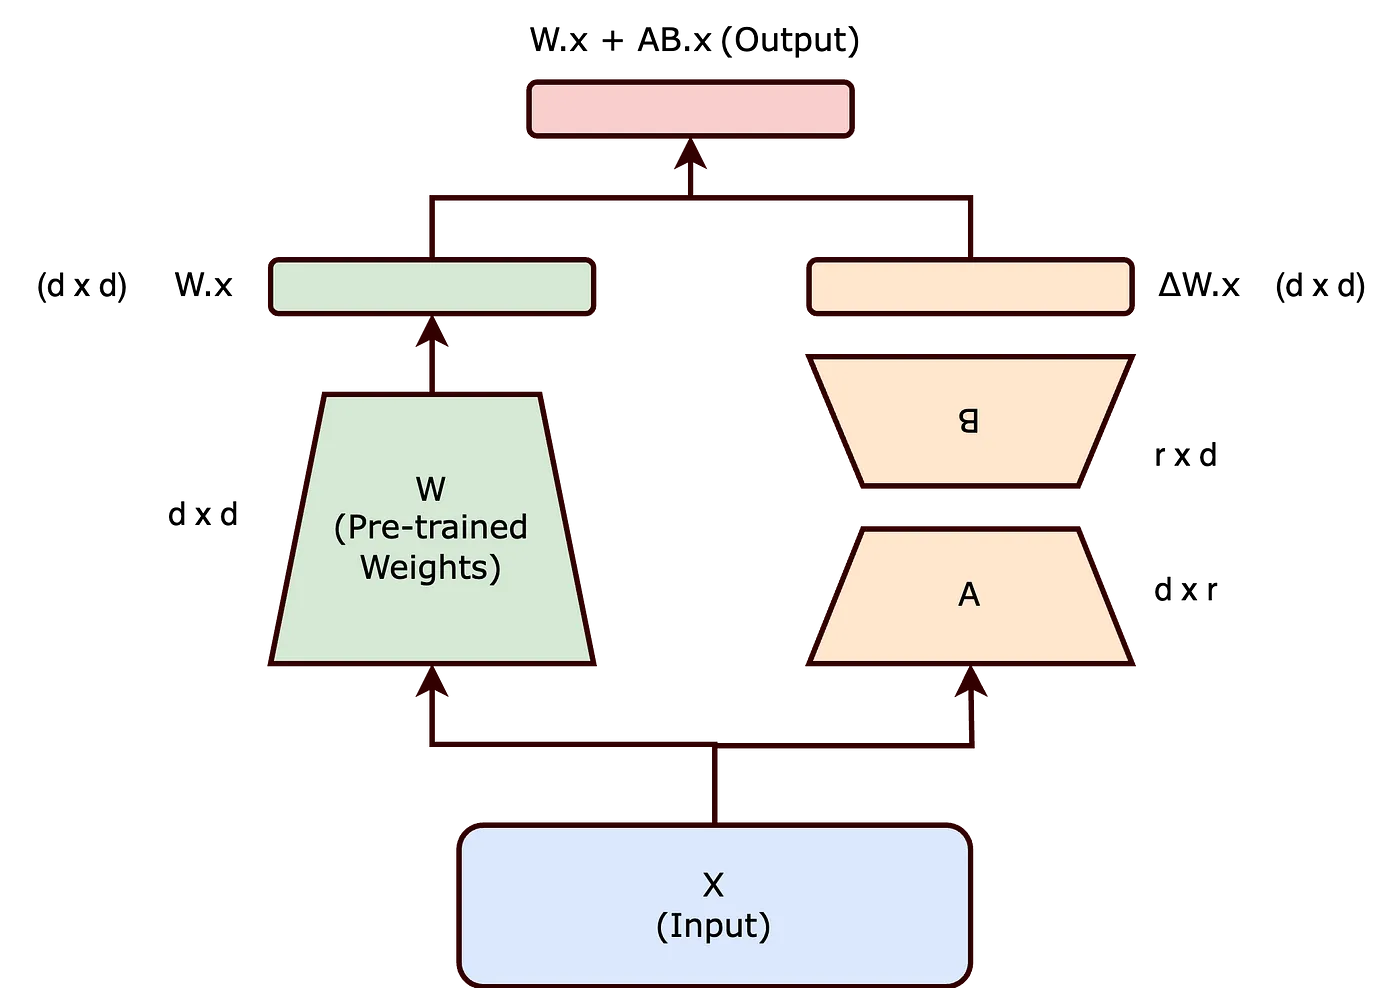
\includegraphics[width=0.8\textwidth]{images/llms/lora.png}
    \caption{Decomposition of \( \Delta W \) into two matrices \( A \) and \( B \), both of lower dimensionality than \( d \times d \). \textit{Source:} \cite{towardsdatascience2024lora}}
    \label{fig:lora_decomposition}
\end{figure}

As illustrated in Figure \ref{fig:lora_decomposition}, by choosing matrices \( A \) and \( B \) to have a lower rank \( r \), the number of trainable parameters is significantly reduced. For instance, if \( W \) is a \( d \times d \) matrix, traditionally, updating \( W \) would involve \( d^2 \) parameters. However, with \( B \) and \( A \) of sizes \( d \times r \) and \( r \times d \) respectively, the total number of parameters reduces to \( 2dr \), which is much smaller when \( r \ll d \) \cite{hu2021lora}. \newline

The reduction in the number of trainable parameters achieved through the LoRA method offers several significant advantages, particularly in the fine-tuning of large-scale neural networks. By lowering the number of parameters that need to be updated, LoRA reduces the system's memory footprint, which is crucial when managing extensive models. This reduction also leads to faster training and adaptation, as the computational demands are significantly diminished, allowing for more efficient training and fine-tuning of models for new tasks. Furthermore, the decreased parameter count makes it feasible to fine-tune large models on less powerful hardware, such as modest GPUs or CPUs, thereby broadening the accessibility of advanced AI capabilities. Finally, LoRA facilitates the scaling of AI models, enabling the expansion of their size and complexity without a corresponding increase in computational resources, thereby making the management of larger models more practical and cost-effective \cite{towardsdatascience2024lora}.

In the context of LoRA, the concept of rank plays a pivotal role in determining the efficiency and effectiveness of the adaptation process. Remarkably, the paper highlights that the rank of the matrices \( A \) and \( B \) can be astonishingly low, sometimes as low as one.

Despite the contributions of Hu et al. \cite{hu2021lora} primarily presents experiments in the field of NLP, the approach of low-rank adaptation is not limited to this domain and could be effectively employed in training various types of neural networks across different domains.

\section{Prompt-based Learning}

Prompt-based learning represents a significant shift in how LLMs are employed for natural language processing tasks. Instead of relying on extensive labeled datasets for training or fine-tuning, prompt-based learning uses textual prompts to guide the model in performing a specific task. This approach is particularly valuable in scenarios where the cost of annotating large datasets is prohibitive, such as in the development of AI chatbots for conversational AI \cite{madotto2021few}.

Prompt-based learning leverages the model's pre-trained knowledge by providing a prompt or instruction that directs the model's responses. The effectiveness of this technique has been demonstrated by works such as Radford et al. (2019) \cite{radford2019language} and Brown et al. (2020) \cite{brown2020language}, where prompt-based few-shot learning achieved results comparable to state-of-the-art models trained with full-shot datasets. This method relies on the model's ability to generalize from minimal examples (few-shot learning) or even without any examples (zero-shot learning), making it a versatile and cost-effective solution for various NLP tasks, including question answering and sentiment analysis.

\subsubsection{Prompt-Based Learning vs. Fine-Tuning}

The primary distinction between prompt-based learning and traditional fine-tuning lies in the training approach. While fine-tuning involves updating the model's weights based on a training set through a defined loss function, requiring substantial computational effort, prompt-based learning eliminates the need for this training phase altogether. Instead of modifying the model, prompt-based learning utilizes pre-defined prompts that instruct the model on how to perform a task without altering its weights. This makes prompt-based learning particularly advantageous in scenarios with limited computational resources or when rapid adaptation to new tasks is required, as it avoids the need for retraining \cite{madotto2021few}. 

\begin{figure}[h]
    \centering
    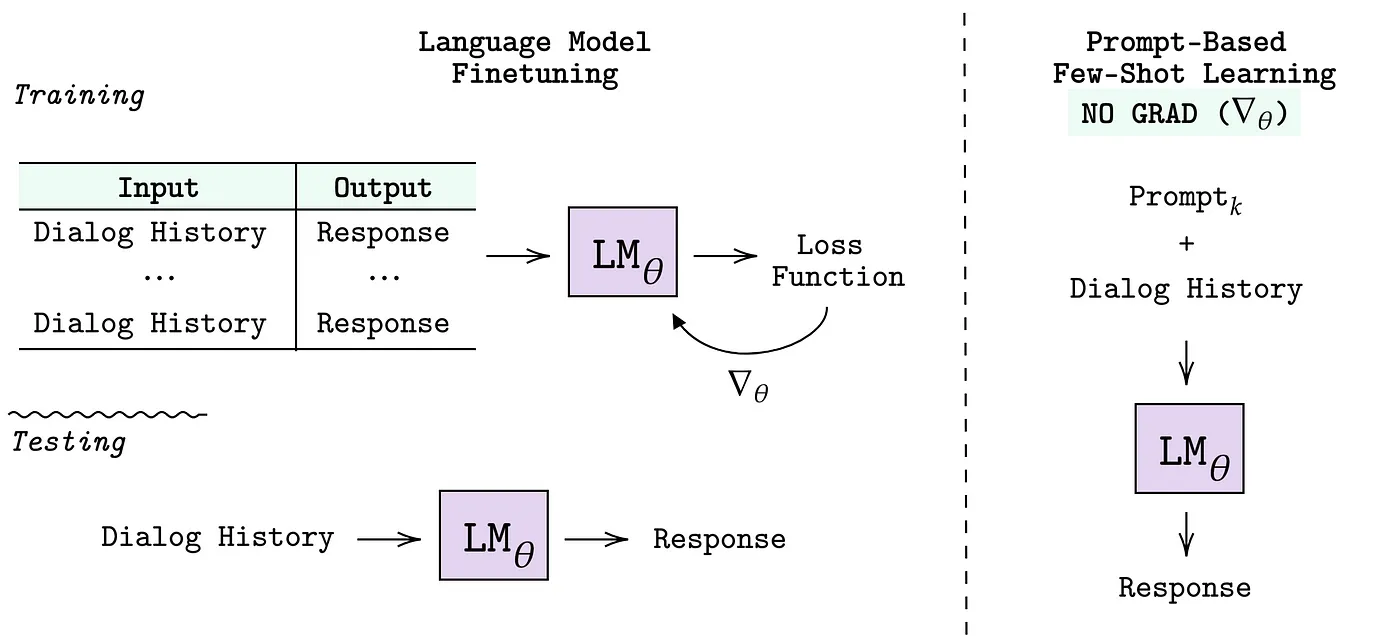
\includegraphics[width=0.8\textwidth]{images/llms/fine-tuning-vs-prompt-learning.png}
    \caption{Comparison of traditional fine-tuning (left) and prompt-based learning (right). In traditional fine-tuning, the model's weights are updated based on a training set, while in prompt-based learning, the model uses pre-defined prompts without altering its weights. \textit{Source:} \cite{madotto2021few}}
    \label{fig:fine_tuning_vs_prompt_learning}
\end{figure}

\subsection{Zero-Shot, One-Shot, and Few-Shot Learning}

Prompt-based learning is often implemented using zero-shot, one-shot, or few-shot prompts, each offering varying levels of example-based guidance to the model.

In Zero-Shot learning, the model is given a prompt to perform a task without any additional examples. The model relies solely on its pre-trained knowledge to generate a response, making zero-shot prompts highly efficient in scenarios where no task-specific data is available \cite{radford2019language}.

One-Shot learning involves providing the model with a single example in addition to the prompt. This example serves as a minimal guide, helping the model to generate responses that align more closely with the desired outcome.

Few-Shot learning extends this approach by supplying the model with a small number of examples (typically more than one but fewer than what would be used in full training). These examples, provided in the context of the prompt, help the model understand the task better, allowing it to produce responses that are more accurate and contextually appropriate \cite{brown2020language}.

\begin{figure}[h]
    \centering
    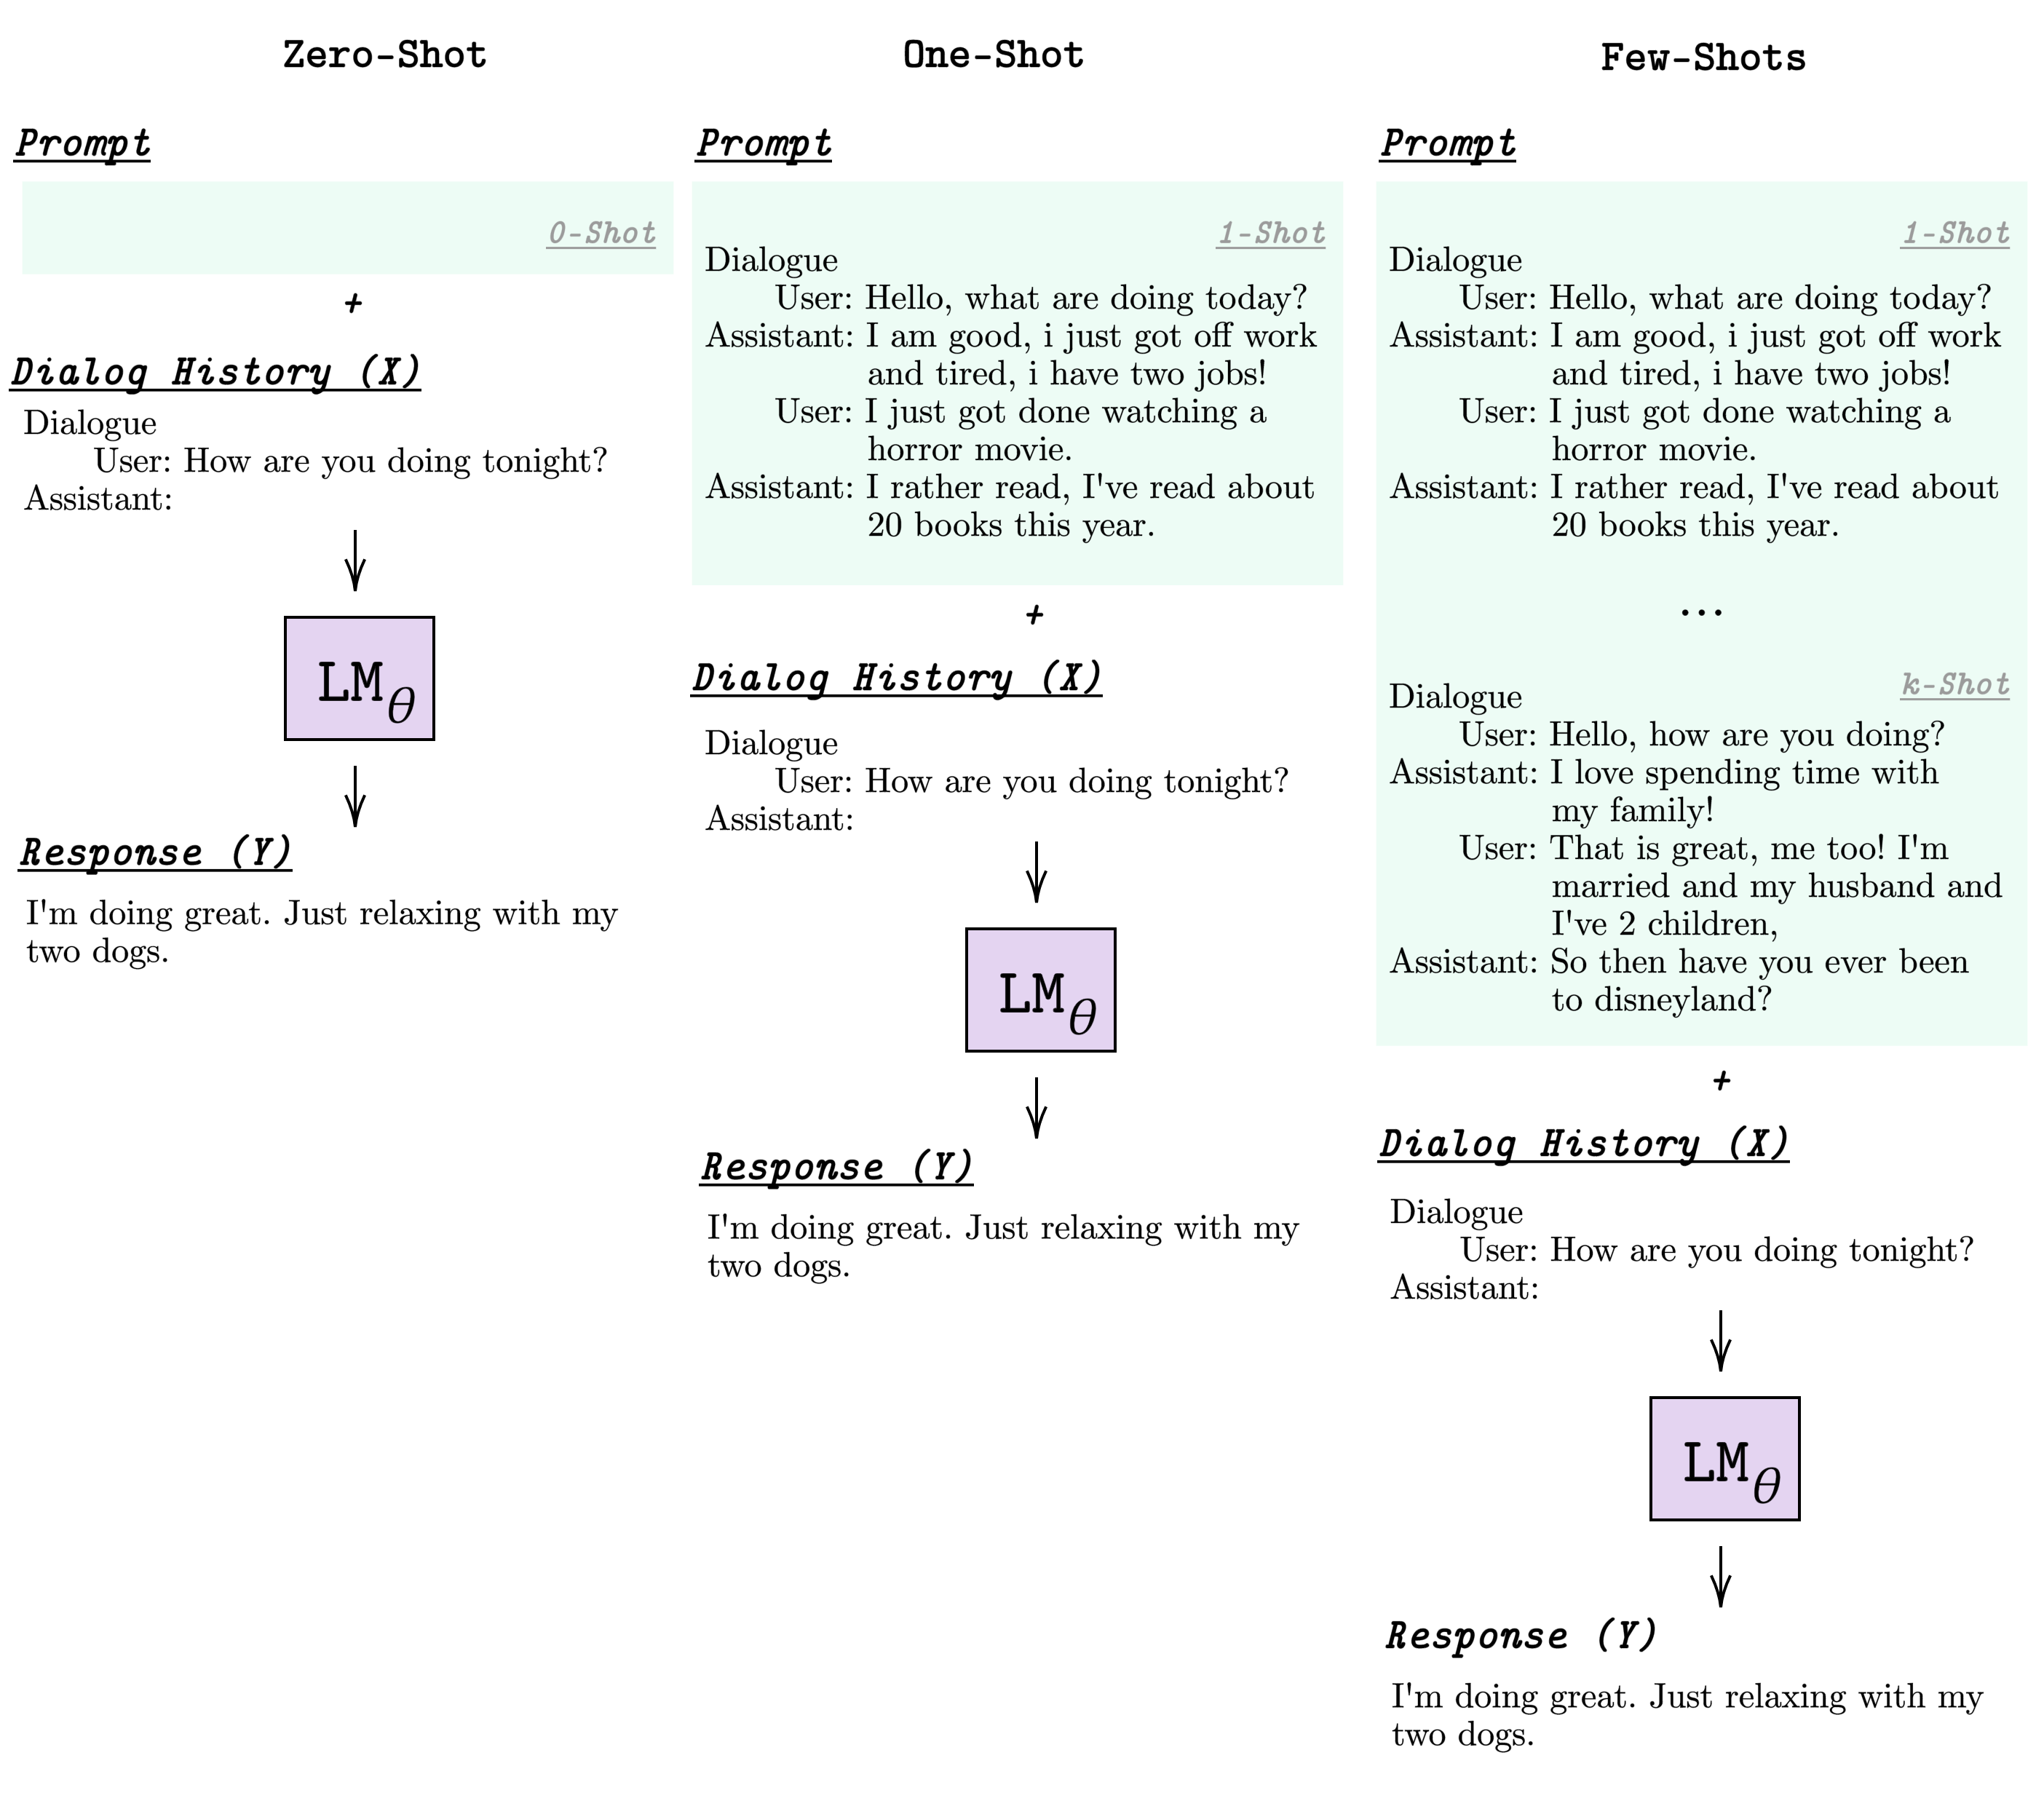
\includegraphics[width=0.8\textwidth]{images/llms/zero-one-few-shots.png}
    \caption{Illustration of Zero-Shot, One-Shot, and Few-Shot learning in dialogue systems. Zero-Shot learning involves no additional examples, One-Shot learning provides a single example, and Few-Shot learning includes a small number of examples to guide the model's response generation. \textit{Source:} \cite{madotto2021few}}
    \label{fig:zero_one_few_shot}
\end{figure}

As illustrated in Figure \ref{fig:zero_one_few_shot}, the effectiveness of prompt-based few-shot learning has been demonstrated across a wide range of tasks, including dialogue response generation, knowledge-grounded response generation, and dialogue state tracking. In many cases, it achieves performance comparable to, or even exceeding, that of fully fine-tuned models, without the need for extensive retraining. This makes prompt-based learning a powerful tool in the deployment of conversational AI systems, where flexibility and efficiency are paramount.

In conclusion, prompt-based learning offers a compelling alternative to traditional fine-tuning by allowing LLMs to perform specific tasks with minimal or no retraining. By utilizing zero-shot, one-shot, and few-shot prompts, this approach maximizes the utility of pre-trained models, making them more adaptable and cost-effective in a wide variety of applications.

\subsection{Chain of Thought Prompting}

In recent years, more advanced techniques have emerged, with one particularly promising approach being Chain-of-Thought (CoT) prompting.

Chain-of-Thought reasoning represents a methodology designed to enhance the reasoning capabilities of large language models by directing them to construct a sequence of intermediate steps that collectively culminate in a final answer. This approach emulates the natural human thought process when addressing complex tasks, such as multi-step mathematical problems, where the problem is decomposed into smaller, more tractable components before reaching a solution.

As illustrated in Figure \ref{fig:cot_reasoning}, Chain of Thought reasoning allows language models to handle complex reasoning tasks more effectively by decomposing the problem into intermediate stages. For example, when solving a math word problem, a model might generate a sequence of logical steps that resemble the way a human might solve the problem step-by-step: “After Jane gives 2 flowers to her mom, she has 10 left… then after giving 3 to her dad, she will have 7… so the answer is 7.” This sequential reasoning helps the model arrive at the correct answer by focusing on each part of the problem individually.

\begin{figure}[h]
    \centering
    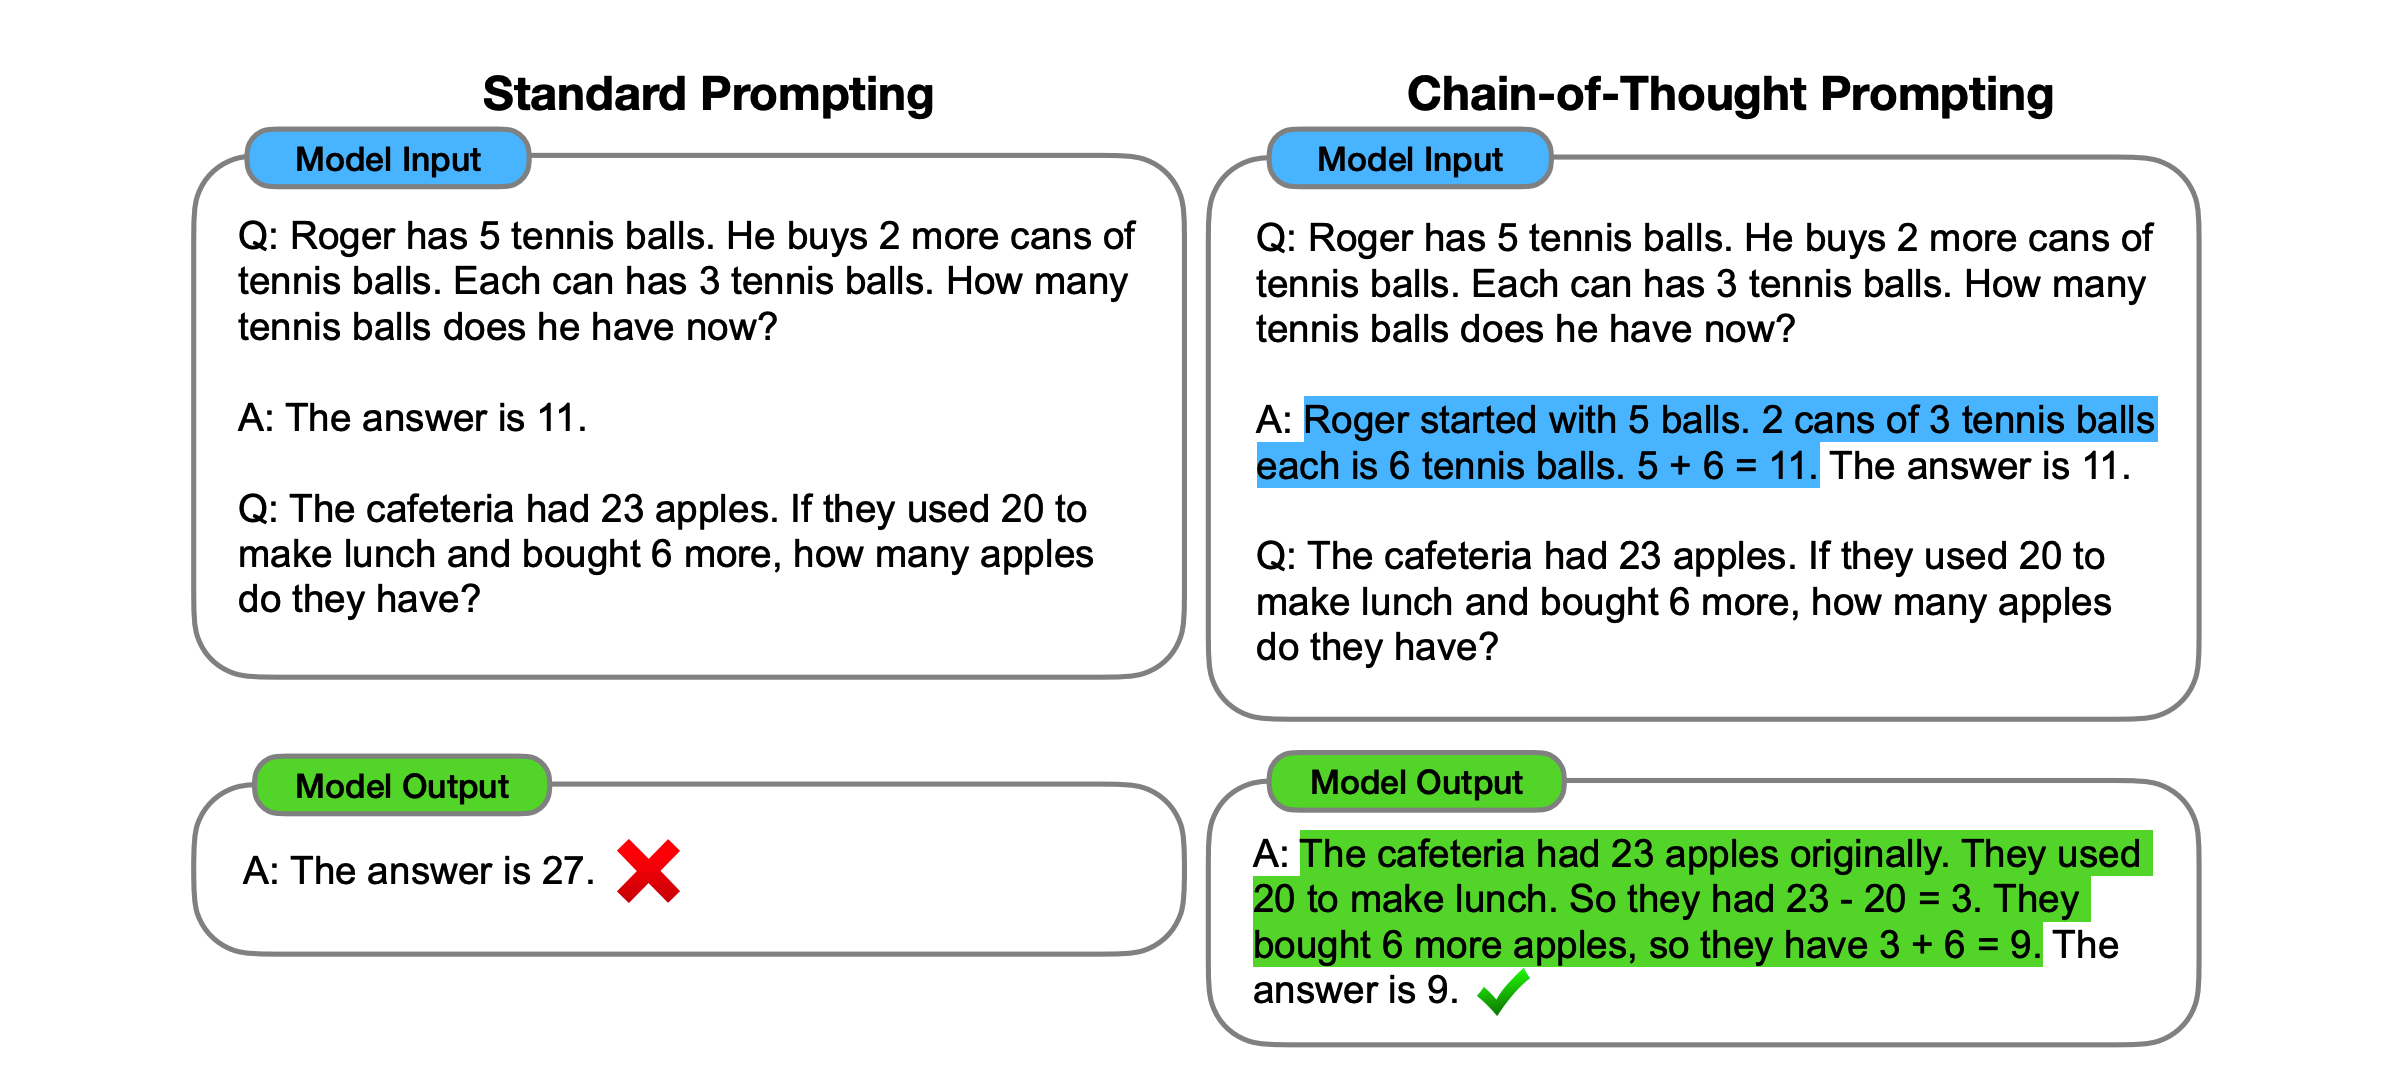
\includegraphics[width=0.8\textwidth]{images/llms/cot-resoning.png}
    \caption{Comparison of standard prompting and Chain-of-Thought (CoT) prompting. The CoT approach allows the model to break down problems into intermediate steps, leading to more accurate and interpretable outcomes.}
    \label{fig:cot_reasoning}
\end{figure}

One of the significant advantages of Chain of Thought reasoning is its interpretability. By breaking down the reasoning process into a series of intermediate steps, CoT provides insights into how the model arrived at a particular answer. This not only helps in understanding the model’s decision-making process but also offers opportunities to identify and correct errors in the reasoning path.

Moreover, Chain of Thought reasoning is versatile and can be applied to a variety of tasks that require complex reasoning, such as solving math word problems, engaging in commonsense reasoning, and performing symbolic manipulation. Essentially, it can be applied to any task where humans typically solve problems through language-based reasoning.

Another notable benefit of Chain of Thought prompting is that it can be effectively elicited in large language models by incorporating examples of such reasoning into the few-shot prompting process. This means that without any additional fine-tuning, sufficiently large pre-trained models can generate these reasoning chains simply by being provided with relevant examples during the prompting phase \cite{wei2022chain}.

In summary, Chain of Thought reasoning represents a powerful tool for enhancing the reasoning capabilities of language models. By breaking down complex problems into intermediate steps, it not only improves the accuracy of the model’s outputs but also provides a transparent and interpretable reasoning process that can be applied across a wide range of tasks.

\subsection{Instruction Prompt Tuning}

% ----------------------- Read from here  -----------------------

An innovative technique, instruction prompt tuning, introduced by Lester et al. \cite{lester2021power}, provides a cost-effective solution to update the model's parameters, thereby improving performance in numerous downstream tasks. Instruction prompt tuning offers significant advantages over few-shot prompting, particularly for clinical applications, because it allows LLMs to be more effectively aligned with the specific requirements of the medical domain, as demonstrated by Singhal et al. \cite{singhal2022large}

Prompt tuning is designed to improve the performance of frozen language models on specific downstream tasks by learning so-called "soft prompts". Unlike traditional discrete text prompts, which are manually selected or searched for, soft prompts are learned through backpropagation, allowing them to be fine-tuned based on labeled examples.

At a high level, prompt tuning shifts the focus from tuning the entire model to tuning only the parameters of the prompts. This approach involves conditioning a frozen language model on these soft prompts to guide its output generation, thereby enhancing the model's ability to perform specific tasks. This is particularly important because it allows the use of large pre-trained models without the need to modify their core weights, making the approach both resource efficient and scalable.

The concept of prompt tuning builds on the idea of conditioning models with additional information. Typically, in models such as GPT-3, prompts are added as additional tokens that the model uses to generate the desired output. However, these tokens are part of the model's fixed embedding space, which means that they cannot be directly optimized by training. Prompt tuning overcomes this limitation by introducing dedicated parameters for the prompts themselves, which can be updated during training.

As a result, prompt tuning becomes increasingly competitive as the size of the language model grows. Remarkably, it can match the performance of full model tuning - where all model weights are adjusted - even when the model size reaches billions of parameters. This makes prompt tuning a powerful tool, especially for large models where fine-tuning all parameters is computationally expensive and impractical.

In addition, prompt tuning has demonstrated advantages in robustness to domain transfer and offers the flexibility of "prompt ensembling," where multiple prompts can be combined to improve performance. This approach also simplifies the process of adapting a single frozen model to multiple downstream tasks, reducing the need to deploy and manage multiple fine-tuned models. \cite{lester2021power}

In summary, prompt tuning is a highly effective method for improving the performance of large language models on specific tasks by learning and tuning soft prompts. This approach not only simplifies the tuning process, but also maintains the efficiency and scalability of using frozen, pre-trained models across different applications. 

\section{Limitations of Large Language Models in Practical Applications}

Review of recent literature on incorporating external knowledge into task-oriented dialogue systems.

After examining LLMs, their architecture, and the impact of model size on AI performance, as well as exploring various training and fine-tuning methods, including prompt-based learning techniques, it is essential to address the limitations of these models in practical applications.

One of the most significant limitations of LLMs is their lack of transparency in predictions. The models operate as black boxes, making it difficult to interpret the reasoning behind their outputs. This opacity is problematic, especially when LLMs are used in decision-making processes that require accountability and traceability \cite{rudin2019stop}.

Another critical issue is the tendency of LLMs to produce “hallucinations”—statements that are plausible but factually incorrect. These hallucinations arise because LLMs generate text based on patterns learned from vast amounts of data, without a deep understanding of the world or the ability to fact-check their outputs \cite{maynez2020faithfulness}. This risk is exacerbated by the fluency and coherence of the generated text, which can mislead users into accepting false information as true.

Bias is another well-documented limitation of LLMs. These models can inadvertently perpetuate and amplify biases present in the training data, leading to outputs that reinforce stereotypes or discriminate against certain groups \cite{bender2021dangers}. This bias is particularly concerning in applications like hiring, lending, or law enforcement, where fairness and impartiality are paramount.

Additionally, LLMs face issues of staleness and revisions. Since these models are trained on static datasets, they cannot incorporate new information that emerges after their training, leading to outdated or incorrect responses \cite{dhingra2022time}. Furthermore, the accuracy of information retrieval is another challenge, as LLMs often struggle to retrieve specific, relevant information from their vast learned knowledge, leading to irrelevant or imprecise responses.

The limitations mentioned above significantly undermine the reliability and value of LLMs in practical applications. When these models generate inaccurate or misleading outputs, the consequences can be severe, especially in critical fields where precision and factual correctness are essential.

To address these limitations, one promising approach is Retrieval-Augmented Generation (RAG). RAG enhances the capabilities of LLMs by integrating an external retrieval mechanism that allows the model to access and utilize up-to-date and contextually relevant information during the generation process \cite{lewis2020retrieval}. This method mitigates issues related to staleness, hallucinations, and factual inaccuracies by grounding the model’s outputs in verifiable external sources, thereby improving the accuracy and reliability of its responses. As a result, RAG offers a viable solution to many of the challenges faced by LLMs in practical applications, making them more effective and trustworthy in real-world scenarios.

\section{Retrieval-Augmented Generation (RAG)}

To address the discussed challenges, Meta AI researchers introduced a method called Retrieval-Augmented Generation (RAG) \cite{lewis2020retrieval}. RAG is a powerful technique that enhances LLMs by integrating them with external knowledge sources, operating by retrieving relevant document chunks from an external knowledge base through semantic similarity calculations. By referencing external knowledge, RAG effectively reduces the occurrence of hallucinations and improves the factual accuracy of the generated content. This integration has led to widespread adoption of RAG, establishing it as a key technology in advancing AI applications like chatbots and enhancing the suitability of LLMs for real-world scenarios.

The development of RAG technology has progressed rapidly, evolving through distinct stages. Initially, the inception of RAG coincided with the rise of the Transformer architecture, focusing on enhancing language models by incorporating additional knowledge through Pre-Training Models (PTM). This early stage was characterized by foundational work aimed at refining pre-training techniques \cite{arora2023gar, lewis2020retrieval, borgeaud2022improving}. 

The subsequent arrival of models like ChatGPT marked a pivotal moment, showcasing powerful in-context learning (ICL) capabilities. RAG research shifted towards providing better information for LLMs to tackle more complex and knowledge-intensive tasks during the inference stage. As research progressed, RAG's enhancement was no longer limited to the inference stage but began to incorporate more with LLM fine-tuning techniques.

A typical application of RAG is illustrated in Figure \ref{fig:rag_example}. In this example, a user poses a question to ChatGPT about a recent news event. Given that ChatGPT relies on pre-training data, it initially lacks the ability to provide updates on recent developments. RAG bridges this information gap by sourcing and incorporating knowledge from external databases. In this case, relevant news articles related to the user's query are retrieved and combined with the original question to form a comprehensive prompt, empowering the LLM to generate a well-informed answer.

\begin{figure}[h]
    \centering
    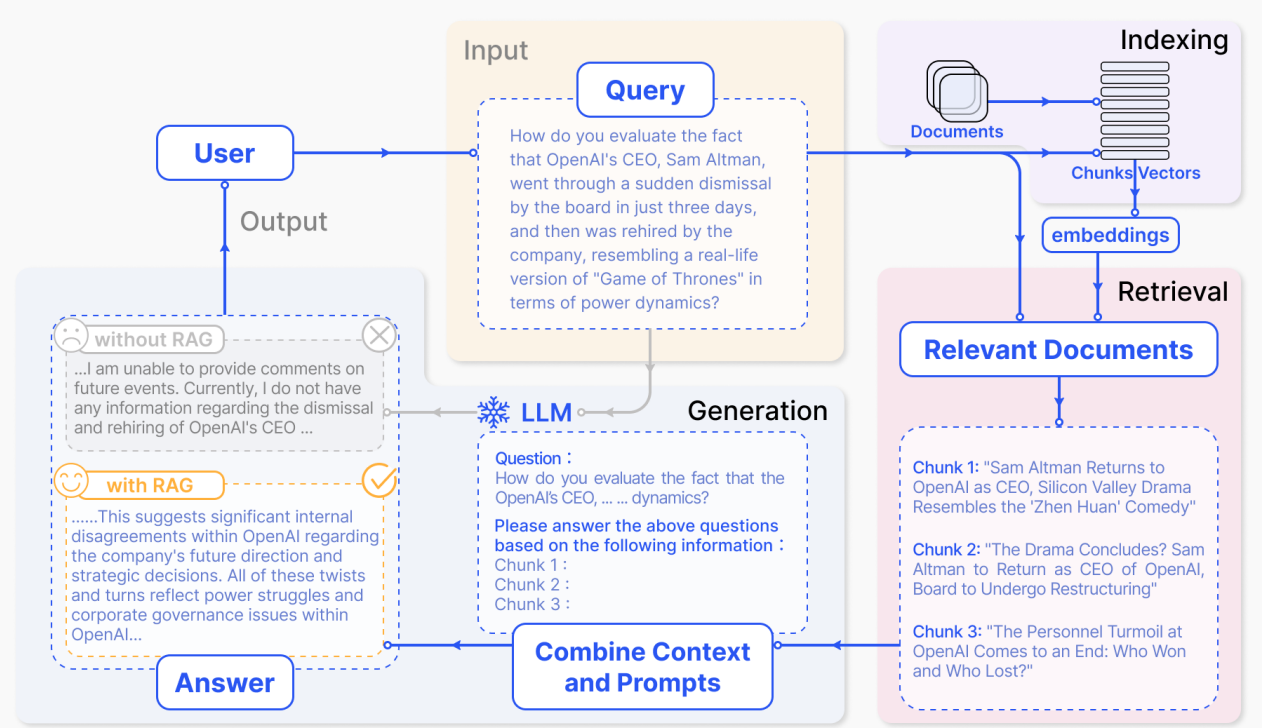
\includegraphics[width=0.8\textwidth]{images/llms/rag-strategies.png}
    \caption{A representative instance of the RAG process applied to question answering. It consists of three main steps: 1) Indexing, where documents are split into chunks, encoded into vectors, and stored in a vector database. 2) Retrieval, where the top-K chunks most relevant to the question are retrieved based on semantic similarity. 3) Generation, where the original question and the retrieved chunks are input together into the LLM to generate the final answer. \textit{Source:} \cite{gao2023retrieval}}
    \label{fig:rag_example}
\end{figure}

As RAG continues to evolve, we can categorize its development into three stages: Naive RAG, Advanced RAG, and Modular RAG. Although RAG methods are cost-effective and surpass the performance of native LLMs, they also exhibit certain limitations. The development of Advanced RAG and Modular RAG represents a response to these specific shortcomings in the Naive RAG stage \cite{gao2023retrieval}.

\subsubsection{Naive RAG}

The Naive Retrieval-Augmented Generation (RAG) approach represents the foundational methodology in RAG systems and gained prominence following the widespread adoption of models like ChatGPT. Naive RAG follows a straightforward "Retrieve-Read" framework \cite{ma2023query}, which typically involves three critical phases: indexing, retrieval, and generation.

\textbf{Indexing} is the initial phase where raw data from various formats, such as PDFs, HTML, Word documents, and Markdown files, are cleaned and converted into a uniform plain text format. Given the context limitations of language models, the text is then segmented into smaller, manageable chunks. These chunks are encoded into vector representations using an embedding model and stored in a vector database. This process is crucial as it lays the groundwork for efficient similarity searches during the retrieval phase.

\textbf{Retrieval} begins when a user query is submitted. The system utilizes the same encoding model used during indexing to transform the query into a vector representation. The system then computes similarity scores between the query vector and the vectors of chunks within the indexed corpus. The top K chunks with the highest similarity scores are retrieved and used as the expanded context for the prompt.

\textbf{Generation} involves synthesizing the user’s query with the retrieved documents to create a coherent prompt, which the large language model uses to generate a response. Depending on task-specific criteria, the model might draw on its parametric knowledge or restrict its response to the retrieved documents. However, Naive RAG faces several significant challenges, including issues with retrieval precision and recall, and the generation of content that may suffer from hallucinations, irrelevance, or bias \cite{gao2023retrieval}.

\subsubsection{Advanced RAG}

Advanced RAG builds on the foundational Naive RAG framework by introducing specific improvements designed to address the limitations observed in the earlier model. This approach enhances the quality of retrieval by implementing both pre-retrieval and post-retrieval strategies, focusing on refining the indexing process and optimizing how queries are handled.

In the pre-retrieval phase, the emphasis is on optimizing the structure of the index and refining the original user query to improve retrieval quality. Strategies such as the sliding window approach, fine-grained text segmentation, and the incorporation of metadata are employed to enhance the granularity and relevance of the indexed content \cite{ilin2023advancedrag}. Additionally, query optimization techniques such as query rewriting, transformation, and expansion are used to ensure the query is well-suited for effective retrieval.

The post-retrieval phase focuses on integrating the retrieved context more effectively with the user’s query. Key methods include re-ranking the retrieved chunks to prioritize the most relevant information and compressing the context to avoid information overload when feeding it into the language model. These strategies help address the generation challenges encountered in Naive RAG by ensuring that the final output is more focused, relevant, and coherent.

Advanced RAG’s systematic enhancements to both the indexing and retrieval processes significantly improve the overall performance of RAG systems, making them more robust and capable of handling complex queries with greater accuracy \cite{gao2023retrieval}.

\subsubsection{Modular RAG}

Modular RAG represents the next evolution in the RAG paradigm, offering a more flexible and adaptable architecture that can be customized to meet the needs of a wide range of tasks and scenarios. This approach builds upon the foundational principles of Naive and Advanced RAG but introduces modular components that can be independently optimized and reconfigured.

\textbf{New Modules} are a key feature of Modular RAG. This architecture incorporates specialized components designed to enhance retrieval and processing capabilities. For instance, the \textbf{Search module} allows for direct searches across diverse data sources, such as search engines, databases, and knowledge graphs, using LLM-generated code and query languages \cite{wang2023knowledgpt}. The \textbf{RAGFusion module} addresses the limitations of traditional search by employing a multi-query strategy that expands user queries into diverse perspectives, utilizing parallel vector searches and intelligent re-ranking to uncover both explicit and transformative knowledge \cite{ragfusion2023}. Additionally, the \textbf{Memory module} leverages the language model’s memory to guide retrieval, creating an unbounded memory pool that iteratively enhances the alignment between text and data distribution \cite{li2021memory}.

The \textbf{Routing module} in Modular RAG optimizes query pathways by navigating through various information sources, selecting the most appropriate route for each query. This might involve summarization, specific database searches, or merging different information streams to provide a comprehensive response \cite{li2023classification}. The \textbf{Predict module} reduces redundancy and noise by generating context directly within the LLM, ensuring that the outputs are relevant and accurate \cite{yu2022generate}. Finally, the \textbf{Task Adapter module} tailors the RAG system to various downstream tasks, automating prompt retrieval for zero-shot inputs and creating task-specific retrievers through few-shot query generation \cite{cheng2023uprise}.

\textbf{New Patterns} in Modular RAG provide remarkable adaptability by allowing for module substitution or reconfiguration to address specific challenges. Unlike the fixed structures of Naive and Advanced RAG, Modular RAG offers the flexibility to integrate new modules or adjust the interaction flow among existing ones, enhancing its applicability across different tasks. Innovations such as the \textbf{Rewrite-Retrieve-Read} model and the \textbf{Demonstrate-Search-Predict} (DSP) framework illustrate how Modular RAG can leverage LLMs capabilities to refine retrieval queries and improve task performance \cite{khattab2022demonstrate}.

Modular RAG’s dynamic architecture not only simplifies the retrieval process but also significantly enhances the quality and relevance of the information retrieved. Its flexibility allows for the integration of other technologies, such as fine-tuning or reinforcement learning, further expanding its effectiveness and adaptability in diverse application scenarios.

\begin{figure}[h]
    \centering
    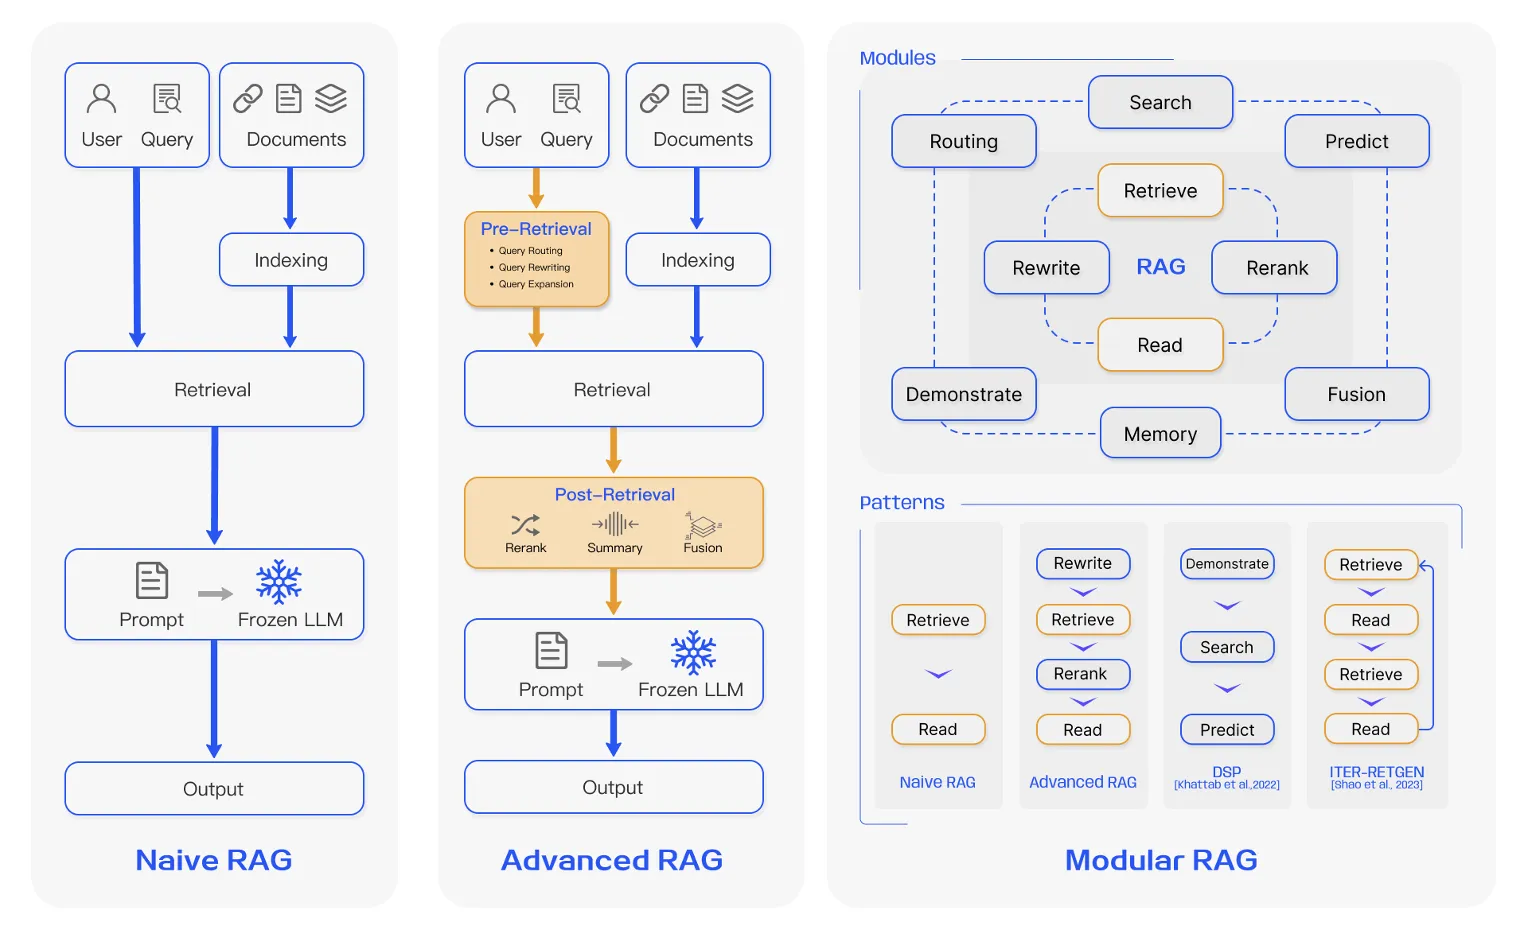
\includegraphics[width=0.8\textwidth]{images/llms/naive-adv-modular-rag.png}
    \caption{Comparison between the three paradigms of RAG. Naive RAG (left) consists of three parts: indexing, retrieval, and generation. Advanced RAG (middle) introduces multiple optimization strategies around pre-retrieval and post-retrieval, while Modular RAG (right) develops from the previous paradigms, showcasing greater flexibility with the introduction of multiple specific functional modules. \textit{Source:} \cite{gao2023retrieval}}
    \label{fig:rag_paradigms}
\end{figure}

In summary, Modular RAG represents a significant advancement in the development of RAG systems, offering a highly adaptable and modular architecture that addresses the limitations of earlier models while providing the flexibility needed to tackle a wide range of complex tasks.

\subsection{Key Considerations for Effective Retrieval in RAG Systems}

In RAG systems, the efficient retrieval of relevant documents from external data sources is critical to ensuring the accuracy and relevance of generated outputs. Several important aspects influence the effectiveness of retrieval, including the source of the retrieval data, the granularity of the data retrieved, indexing optimization, query optimization, and embedding techniques.

\subsection{Retrieval Source}

RAG systems leverage external knowledge sources to enhance LLMs. The type of retrieval source and the granularity of retrieval units significantly impact the quality of the final output.

For open-domain question-answering (ODQA) tasks, traditional unstructured text, such as Wikipedia or domain-specific data, remains the most common retrieval source. In addition to encyclopedic data, common unstructured data inlcudes cross-lingual text and domain specific-data \cite{li2023classification}.

However, RAG systems are increasingly incorporating semi-structured data, that typically refers to data that includes both text and table elements, such as PDF files. Managing semi-structured data presents challenges for conventional RAG systems for two main reasons. First, the process of text splitting can unintentionally separate tables, leading to data corruption during retrieval. Second, integrating tables into the data complicates semantic similarity searches. One approach to handling semi-structured data is to utilize the coding capabilities of LLMs to execute Text-2-SQL queries on tables within databases, as seen in systems like TableGPT \cite{zha2023tablegpt}. Alternatively, tables can be converted into text format for further analysis using text-based methods \cite{luo2023augmented}. However, these methods are not without limitations, highlighting the need for further research in this area.

Structured data, such as knowledge graphs (KGs), typically undergoes verification and can provide more precise information. For example, KnowledGPT \cite{wang2023knowledgpt} generates knowledge base search queries and stores knowledge in a personalized repository, enriching the RAG model’s information base. To address the limitations of LLMs in understanding and answering questions related to textual graphs, G-Retriever \cite{he2024g} integrates Graph Neural Networks (GNNs), LLMs, and RAG, thereby enhancing graph comprehension and question-answering capabilities through soft prompting. However, managing structured data requires considerable effort to build, validate, and maintain structured databases.

\subsubsection{Retrieval Granularity}

The granularity of the retrieved data - whether it is at the token, sentence, or document level - plays a crucial role in the retrieval process. Coarse-grained units might provide more context but can introduce irrelevant information, while fine-grained units increase retrieval precision but might lack necessary context. The choice of retrieval granularity should be tailored to the specific downstream tasks to ensure both relevance and coherence in the generated outputs \cite{gao2023retrieval}.

\subsection{Indexing Optimization}

Indexing is a crucial phase in the Retrieval-Augmented Generation (RAG) system, where documents are processed, segmented, and transformed into embeddings that are stored in a vector database. The quality and structure of the indexing process directly impact the effectiveness of subsequent retrieval operations, as they determine whether the correct and most relevant context can be retrieved when needed.

\subsubsection{Chunking Strategy}

A common method for indexing involves splitting the document into smaller segments or "chunks," typically based on a fixed number of tokens (e.g., 100, 256, or 512 tokens) \cite{teja2023chunk}. The choice of chunk size is a balancing act: larger chunks can capture more context, but they also introduce more noise, increasing processing time and computational costs. Conversely, smaller chunks reduce noise but may fail to fully convey the necessary context, potentially leading to incomplete or fragmented retrieval results.

To address these challenges, various optimization strategies have been proposed. For example, recursive splitting and sliding window methods allow for layered retrieval, where globally related information is merged across multiple retrieval processes \cite{langchain2023recursive}. These techniques aim to preserve semantic completeness while accommodating the constraints of context length. However, even with these optimizations, striking the right balance between semantic integrity and context length remains a complex task. Recently, methods like Small2Big have been introduced, where sentences (small units) are used as the retrieval unit, and the preceding and following sentences are provided as (big) context to the LLMs \cite{yang2023smalltobig}. This approach helps in maintaining a coherent context while minimizing noise.

\subsubsection{Metadata Attachments}

In addition to chunking, attaching metadata to chunks can significantly enhance the retrieval process. Metadata may include information such as page numbers, file names, authors, categories, timestamps, and other contextual markers. By embedding this metadata within the index, retrieval can be filtered based on these attributes, narrowing the search scope and improving the relevance of the retrieved information. 

For instance, assigning different weights to document timestamps during retrieval can enable time-aware RAG, ensuring the freshness of the knowledge and preventing the use of outdated information. Moreover, metadata can be artificially constructed. One innovative approach is Reverse HyDE, where hypothetical questions are generated using LLMs based on the document content. During retrieval, the system calculates the similarity between the original query and the hypothetical questions, thereby reducing the semantic gap between the user's question and the answers provided \cite{gao2023retrieval}.

\subsubsection{Structural Indexing}

Another effective method for optimizing indexing is the construction of a hierarchical structure for the documents. In a hierarchical index, documents are arranged in parent-child relationships, with individual chunks linked to these hierarchical nodes. Data summaries are stored at each node, which assists in the swift traversal of data and helps the RAG system determine which chunks to extract. This hierarchical approach not only speeds up the retrieval process but also mitigates issues such as data fragmentation and the illusion caused by block extraction \cite{gao2023retrieval}.

In addition, Knowledge Graphs (KGs) can be integrated into the indexing structure to maintain consistency and enhance retrieval accuracy. KGs delineate the connections between different concepts and entities, reducing the potential for retrieval errors or hallucinations. For instance, the KGP method constructs an index between multiple documents using a KG, where nodes represent paragraphs or structures within documents (e.g., pages, tables), and edges indicate semantic or lexical similarities between these nodes \cite{wang2024knowledge}. This approach addresses challenges in knowledge retrieval and reasoning within a multi-document environment, ensuring that the retrieval process remains coherent and contextually accurate.

Overall, optimizing the indexing phase in RAG systems is vital for ensuring that the retrieval process is efficient, accurate, and capable of delivering the most relevant information to support the generation tasks of large language models.

\subsection{Query Optimization}

One of the primary challenges in RAG systems is effectively leveraging the user's query to retrieve the most relevant information. Naive RAG systems often rely directly on the user’s original query, which may not always be well-formed, precise, or optimized for retrieval purposes. Query optimization involves enhancing the query to improve retrieval effectiveness, ensuring that the system retrieves the most relevant context for generating accurate and coherent responses. This optimization process can be broken down into several key strategies: query expansion, query transformation, and query routing.

\subsubsection{Query Expansion}

Query expansion enriches the original query by generating additional sub-queries, ensuring the retrieval process captures all necessary nuances. Techniques like \textbf{multi-query generation} expand the original query into multiple related queries, executed in parallel to provide a comprehensive context. Another strategy, \textbf{sub-query planning}, breaks down complex queries into simpler sub-queries, improving accuracy and completeness \cite{zhou2022least}. Additionally, \textbf{Chain-of-Verification (CoVe)} validates expanded queries to reduce hallucinations of LLMs, enhancing the reliability of the retrieved information \cite{dhuliawala2023chain}.

\subsubsection{Query Transformation}

Query transformation modifies the original query to improve retrieval suitability. \textbf{Query rewriting} rephrases queries for better compatibility with the retrieval system, while \textbf{hypothetical document embedding} (HyDE) uses LLMs to generate hypothetical documents, focusing retrieval on embedding similarity between generated and real documents \cite{gao2022precise}. \textbf{Step-back Prompting} abstracts the query to create a high-level concept question, combining it with the original query for more accurate results \cite{zheng2023take}.

\subsubsection{Query Routing}

Query routing directs queries through different retrieval pipelines based on their nature. \textbf{Metadata Routing/Filtering} uses extracted keywords to narrow the search scope, while \textbf{Semantic Routing} leverages the semantic content of the query to select the most appropriate retrieval pathway. In some cases, a hybrid approach combines both methods for enhanced routing.

By optimizing queries through expansion, transformation, and routing, RAG systems can retrieve more accurate and contextually relevant information, resulting in higher quality outputs \cite{gao2023retrieval}.

\subsection{Embedding Techniques}

Embeddings play a central role in the retrieval process of RAG systems, as they represent the semantic content of queries and document chunks in a mathematical form that can be compared for similarity. The choice and optimization of embedding models are crucial for ensuring the accuracy and efficiency of the retrieval process. The two primary approaches to embeddings in RAG systems are sparse and dense embeddings, with recent advances introducing hybrid models and fine-tuning techniques to enhance performance.

\subsubsection{Sparse vs. Dense Embeddings}

Sparse embeddings, typically derived from traditional information retrieval models like BM25, represent documents as high-dimensional vectors where each dimension corresponds to a term in the vocabulary. These models excel in capturing term frequency and inverse document frequency (TF-IDF) relationships but may struggle with capturing the semantic nuances of language.

Dense embeddings, on the other hand, are generated by neural models such as BERT, which transform text into dense, low-dimensional vectors that encapsulate the semantic meaning of the text. These embeddings are more effective at capturing the contextual relationships between words, making them well-suited for tasks requiring a deep understanding of language semantics.

\textbf{Hybrid Retrieval Approaches} combine the strengths of both sparse and dense embeddings. In such systems, sparse embeddings are often used to provide an initial set of candidate documents, which are then re-ranked using dense embeddings to refine the retrieval results. This approach leverages the complementary strengths of both embedding types, improving the robustness and accuracy of the retrieval process. For instance, hybrid models have been shown to enhance the zero-shot retrieval capability of dense retrievers by providing a broader context through initial sparse retrievals \cite{gao2023retrieval}.

\subsubsection{Fine-Tuning Embedding Models}

Fine-tuning embedding models is essential in scenarios where the retrieval context significantly deviates from the pre-training corpus, particularly in specialized domains such as healthcare, legal practice, and other fields with proprietary jargon. Fine-tuning involves adjusting the embedding model on a domain-specific dataset to better capture the nuances and specialized knowledge required for effective retrieval in that domain.

In addition to domain-specific fine-tuning, another key purpose of fine-tuning is to align the retriever and generator within the RAG system. This can be achieved by using the outputs of the language model (LM) as a supervision signal for fine-tuning, a process known as \textbf{LM-supervised Retriever} (LSR). This approach ensures that the embeddings generated by the retriever are closely aligned with the generative tasks of the LLM, leading to more coherent and contextually relevant outputs \cite{gao2023retrieval}.

Recent advancements in embedding techniques, such as Reinforcement Learning from Human Feedback (RLHF), involve utilizing LM-based feedback to reinforce the retriever through reinforcement learning. This approach allows the retriever to continuously improve based on real-world feedback, further enhancing the robustness and accuracy of the retrieval process.

Embedding techniques are foundational to the success of RAG systems. By carefully selecting, fine-tuning, and combining embedding models, RAG systems can achieve higher retrieval accuracy, better alignment with generative tasks, and ultimately more reliable and contextually appropriate outputs \cite{gao2023retrieval}.

\subsection{Generation}

After the retrieval phase in a RAG system, directly feeding all retrieved information into a large language model (LLM) for generating responses is generally not ideal. This section discusses the necessary adjustments from two perspectives: optimizing the retrieved content and fine-tuning the LLM itself.

\subsubsection{Context Curation}

Redundant information and overly long contexts can interfere with the LLM’s ability to generate accurate and relevant answers. This phenomenon, known as the “Lost in the middle” problem, occurs when LLMs, like humans, tend to focus primarily on the beginning and end of long texts while neglecting the middle portion. Therefore, it is essential to process the retrieved content effectively before feeding it to the LLM \cite{liu2024lost}.

To address this issue, one effective strategy is reranking, which reorders document chunks to prioritize the most relevant information. By reducing the document pool to a manageable size, reranking enhances retrieval accuracy and refines the inputs for the LLM. This process can be achieved through rule-based methods using metrics like diversity and relevance, or by employing specialized reranking models, such as those from the BERT series or general LLMs like GPT \cite{gao2023chat}.

However, simply reranking documents may not be enough to ensure optimal performance. In fact, contrary to the belief that more relevant documents lead to better results, adding too many documents can introduce noise and diminish the LLM’s focus on key information. To further refine the input, Context Compression techniques can be employed. These techniques use smaller language models (SLMs) to filter out unimportant tokens, transforming the context into a form optimized for LLM processing. This approach balances language integrity with compression efficiency. Additionally, reducing the number of documents in the prompt improves accuracy, as shown by the “Filter-Reranker” paradigm, which combines the strengths of SLMs and LLMs to enhance information extraction tasks. Furthermore, having the LLM critique retrieved content before generating an answer can further boost relevance and accuracy, as demonstrated in applications like Chatlaw \cite{gao2023retrieval, cui2023chatlaw}.

\subsubsection{LLM Fine-tuning}

While context curation is crucial for optimizing the input provided to the LLM, fine-tuning the LLM itself can yield even more significant improvements in performance. Fine-tuning LLMs based on specific scenarios and data characteristics allows for targeted adjustments that incorporate additional knowledge, adapt to particular data formats, and generate responses in a desired style \cite{du2022retrieval}.

Moreover, aligning LLM outputs with human preferences or retriever preferences through reinforcement learning offers another layer of optimization. By manually annotating generated answers and using these annotations as feedback during reinforcement learning, the model can be further refined to better meet the needs of specific tasks. Additionally, when access to powerful proprietary models is limited, distillation methods can be employed to transfer knowledge from more advanced models (e.g., GPT-4) to less powerful ones, ensuring that even smaller models can benefit from the strengths of larger counterparts \cite{shi2023dual}.

\subsection{Augmentation Process in RAG}

The standard practice in Retrieval-Augmented Generation (RAG) often involves a single retrieval step followed by text generation. While this approach is straightforward, it can be insufficient for complex tasks that require multi-step reasoning, as it provides a limited scope of information \cite{yoran2023making}. To address this limitation, several augmentation strategies have been developed to enhance the retrieval process, offering more robust and contextually relevant outputs.

As illustrated in Figure \ref{fig:rag_augmentation}, these augmentation strategies are categorized into three main types: Iterative Retrieval, Recursive Retrieval, and Adaptive Retrieval. Each method provides unique advantages that help improve the retrieval and generation process in RAG systems.

\subsubsection{Iterative Retrieval}

Iterative retrieval involves repeatedly searching the knowledge base based on the initial query and the text generated so far. This process enables the LLM to access a broader and more comprehensive knowledge base, which in turn improves the robustness of the generated responses by providing additional contextual references through multiple retrieval iterations. However, iterative retrieval may introduce challenges such as semantic discontinuity and the accumulation of irrelevant information.

\subsubsection{Recursive Retrieval}

To build upon the iterative approach, Recursive retrieval is employed to improve the depth and relevance of search results by iteratively refining search queries based on the outcomes of previous searches. This approach is particularly useful in complex scenarios where user needs are not fully clear or where the information sought is highly specialized. By incorporating a feedback loop, recursive retrieval gradually converges on the most pertinent information. Additionally, recursive retrieval can be combined with multi-hop retrieval techniques to process data hierarchically, summarizing sections of documents before refining the search further within the document \cite{gao2023retrieval}.

\subsubsection{Adaptive Retrieval}

Further refining the RAG framework, Adaptive retrieval methods enable language models to autonomously determine the optimal timing and content for retrieval, enhancing both the efficiency and relevance of the information sourced. This approach represents a shift towards more active judgment by the language models, where the models, like in Self-RAG \cite{asai2023self}, proactively decide when to initiate retrieval based on the confidence levels in the generated output. Techniques such as "reflection tokens" allow the model to introspect and trigger retrieval only when necessary, thus optimizing the retrieval cycle and ensuring that the model generates the most accurate and relevant responses possible.

\begin{figure}[h]
    \centering
    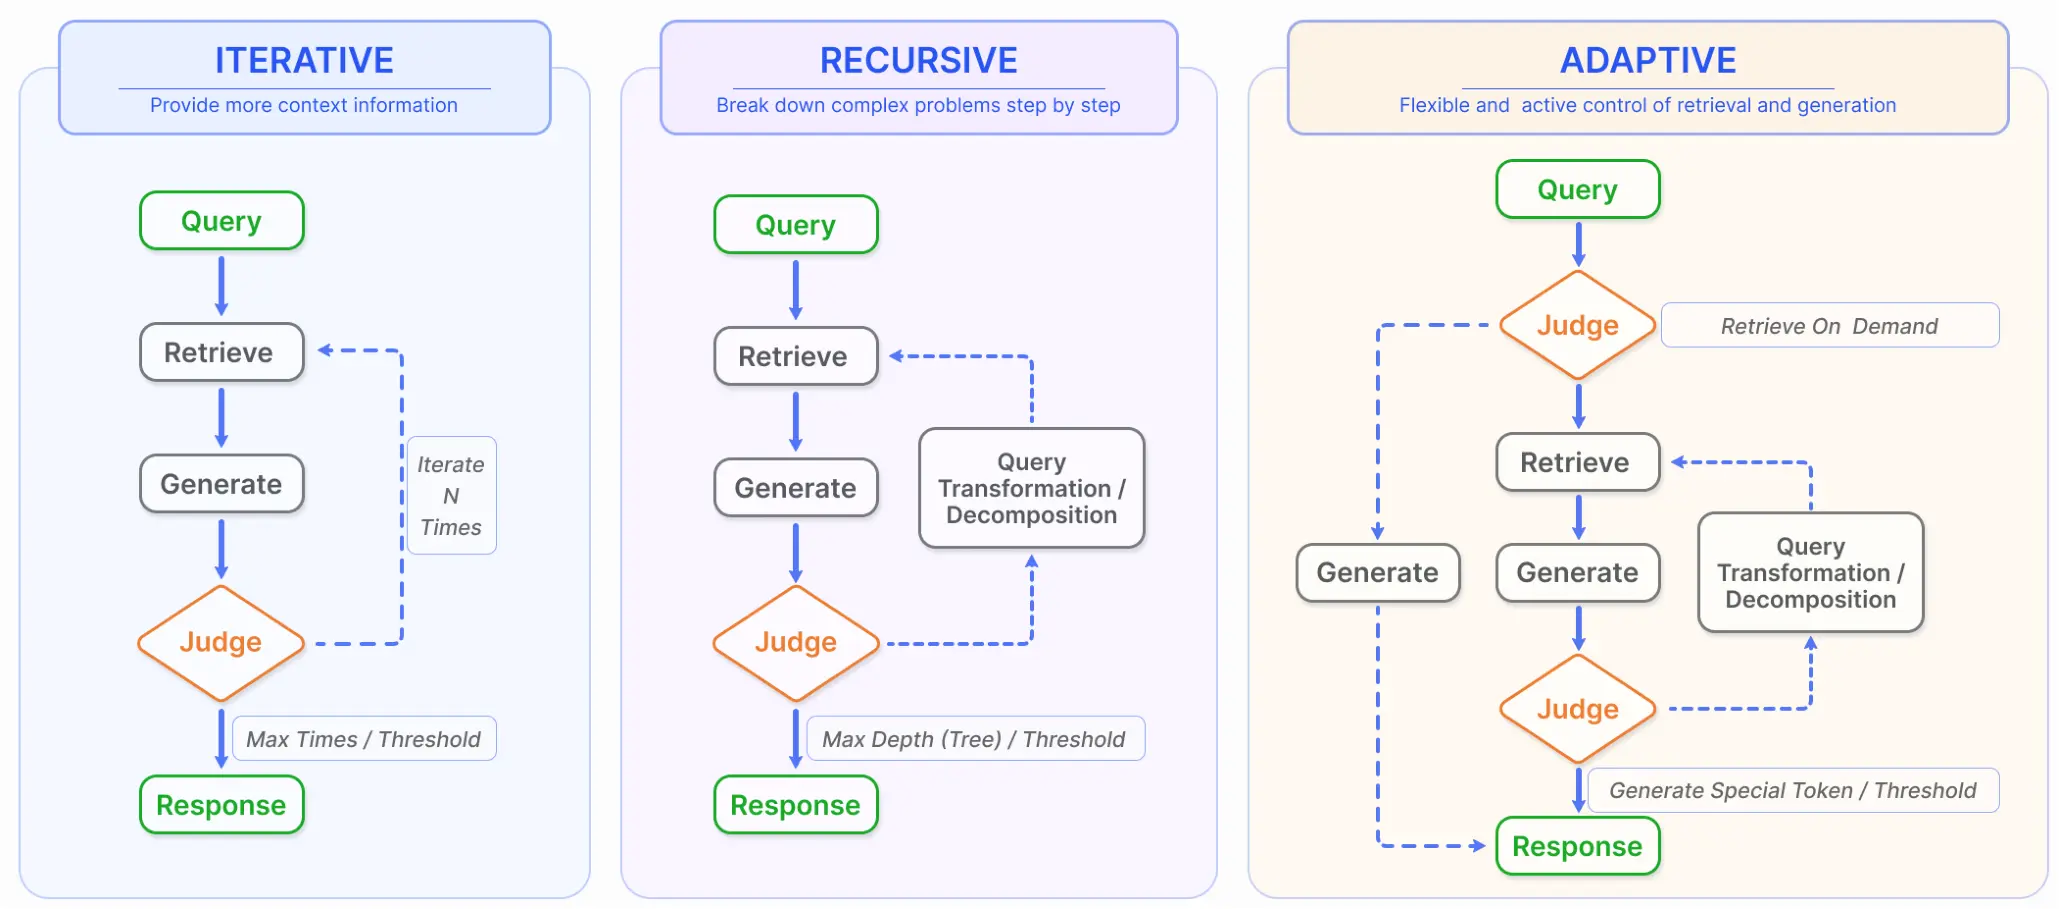
\includegraphics[width=0.8\textwidth]{images/llms/augmentation-process.png}
    \caption{In addition to the most common once retrieval, RAG also includes three types of retrieval augmentation processes. (Left) Iterative retrieval involves alternating between retrieval and generation, allowing for richer and more targeted context from the knowledge base at each step. (Middle) Recursive retrieval involves gradually refining the user query and breaking down the problem into sub-problems, then continuously solving complex problems through retrieval and generation. (Right) Adaptive retrieval focuses on enabling the RAG system to autonomously determine whether external knowledge retrieval is necessary and when to stop retrieval and generation, often utilizing LLM-generated special tokens for control. \textit{Source:} \cite{gao2023retrieval}}
    \label{fig:rag_augmentation}
\end{figure}

In summary, these advanced retrieval strategies—iterative, recursive, and adaptive retrieval—are crucial in addressing the limitations of traditional RAG systems. By refining how and when retrieval occurs, these methods significantly improve the depth, relevance, and accuracy of the information used in generating responses, making RAG systems more capable of handling complex, knowledge-intensive tasks.

\subsection{Future Prospects of RAG Technology}

The field of Retrieval-Augmented Generation (RAG) has seen significant advancements, yet several challenges and opportunities for further research remain. This section discusses the future prospects of RAG technology, focusing on its potential developments and the challenges that must be addressed.

\subsubsection{RAG and Long Contexts}

As research into Large Language Models (LLMs) continues to evolve, the ability of these models to handle increasingly long contexts has improved dramatically. Modern LLMs can effectively handle contexts up to 32,000 tokens, with the industry now moving towards managing contexts of up to 128,000 tokens—equivalent to the length of a 250-page book \cite{ibm2023}. This capability raises questions about the continued relevance of RAG, particularly in tasks such as long-document question answering, where it might seem feasible to input entire documents directly into the model. However, RAG retains its value for several reasons. Firstly, providing an LLM with an excessive amount of context in a single prompt can severely impact inference speed, whereas chunked retrieval and on-demand input significantly enhance operational efficiency. Secondly, RAG-based generation allows for the quick location of original references, enabling users to verify the generated answers. The entire retrieval and reasoning process in RAG is transparent, unlike generation that relies solely on long contexts, which remains a black box. The expansion of context capabilities also opens new avenues for RAG, particularly in tackling complex integrative tasks that require synthesizing information from extensive material. Developing new RAG methods for super-long contexts represents a promising area of future research \cite{gao2023retrieval}.

\subsubsection{Enhancing RAG Robustness}

The presence of noise or contradictory information in the retrieved documents can negatively impact the quality of RAG outputs, leading to the adage that "misinformation can be worse than no information at all." Studies have shown that including irrelevant documents can paradoxically improve accuracy by over 30\%, contradicting the assumption that such inclusion would reduce quality. These findings highlight the need for specialized strategies that integrate retrieval with language generation models more effectively \cite{cuconasu2024power}. Addressing the robustness of RAG systems in the face of noisy or misleading data remains a critical challenge for future research.

\subsubsection{Hybrid Approaches: Combining RAG with Fine-Tuning}

Integrating RAG with fine-tuning techniques is emerging as a powerful strategy for improving model performance. Future research should explore the optimal ways to combine RAG and fine-tuning, whether through sequential, alternating, or end-to-end joint training approaches \cite{lin2023ra}. Another promising avenue is the incorporation of smaller, specialized language models (SLMs) within the RAG framework, where these models can be fine-tuned based on RAG outcomes. For instance, the CRAG model trains a lightweight retrieval evaluator to assess the overall quality of the retrieved documents, triggering different knowledge retrieval actions based on confidence levels \cite{yan2024corrective}. These hybrid approaches offer exciting possibilities for enhancing the efficiency and effectiveness of RAG systems.

\subsubsection{Production-Ready RAG}

The practical application of RAG technology in production environments presents several engineering challenges that must be addressed to enhance its adoption. Key areas of focus include improving retrieval efficiency, enhancing document recall in large knowledge bases, and ensuring data security—such as preventing the inadvertent disclosure of sensitive information by LLMs \cite{alon2022neuro}. The development of the RAG ecosystem is heavily influenced by advancements in its technical stack. Tools like LangChain and LLamaIndex have become integral components of the RAG landscape, offering extensive APIs and user-friendly interfaces. As RAG continues to evolve, there is a clear trend toward specialization, customization, and simplification of RAG tools and platforms.

In chapter 4 of this thesis, I will delve into a case study of RAG application in a production environment by examining WISE, a proprietary chatbot developed by HPA. WISE utilizes the Retrieval-Augmented Generation (RAG) framework to significantly enhance its information retrieval capabilities, offering a sophisticated and efficient solution across various applications. This showcases the effectiveness and reliability of RAG solutions in today’s business landscape.

\subsubsection{Multi-Modal RAG}

RAG technology is rapidly evolving beyond text-based applications to incorporate multi-modal data, resulting in the creation of innovative models that integrate RAG concepts across various domains. In image processing, audio, video, and even code-related tasks, RAG is being used to enhance capabilities such as retrieval, generation, and automatic processing. This expansion into multi-modal domains marks a significant advancement in the development and application of RAG technology, broadening its impact and utility across diverse fields \cite{gao2023retrieval}.

\newline

The future prospects of RAG technology are both promising and complex. As RAG continues to evolve, it will be essential to address the challenges of robustness, scaling, and production readiness while exploring new frontiers in multi-modal applications. The ongoing development of hybrid approaches and the potential for breakthroughs in scaling laws offer exciting opportunities for advancing RAG systems. With continued research and innovation, RAG technology is poised to become an even more integral part of the AI landscape, enabling more efficient, accurate, and versatile applications across a wide range of domains.

\section{Evaluation of LLMs}

% inserire introduzione all'argomento, perché è importante e cosa centra con il resto

This section delves into the evaluation of Large Language Models (LLMs) in the context of the two key areas addressed in this thesis: Natural Language Generation (NLG) and Retrieval-Augmented Generation (RAG). While NLG and RAG share certain evaluation methodologies, the unique objectives and demands of each task require tailored approaches and metrics. This section examines the evaluation techniques for both NLG and RAG, emphasizing their distinct challenges and the innovations that have been developed to address them.

Evaluating NLG has traditionally relied on surface-level metrics such as BLEU \cite{papineni2002bleu} and ROUGE \cite{lin2004rouge}, which assess the n-gram overlap between the model-generated text and reference texts. These metrics have long been used due to their simplicity and ease of application. BLEU, for instance, measures the precision of n-grams in the generated text against a set of reference texts, while ROUGE focuses on recall, particularly in the context of summarization tasks. Despite their widespread use, these metrics have faced criticism for their inability to capture the deeper semantic quality of text, often leading to low correlation with human judgments \cite{sulem2018bleu}.

\subsection{Model-Based Evaluation Metrics}

With the advent of deep learning, more sophisticated evaluation metrics were introduced, such as BERTScore and BARTScore \cite{zhang2019bertscore, yuan2021bartscore}. These metrics leverage pre-trained language models to evaluate generated text by considering various aspects like fluency, coherence, and faithfulness. BERTScore, for example, computes the similarity between the embeddings of the generated and reference texts, offering a more nuanced assessment than n-gram overlap. BARTScore goes a step further by considering the conditional probability of the generated text given the source text, thus evaluating how likely the generated content would be produced by a high-quality language model.

While these model-based metrics offer significant improvements over traditional methods, they are not without their limitations. Their reliance on reference texts limits their applicability in scenarios where references are unavailable. Additionally, these methods, though more aligned with human judgments, still struggle with certain aspects of text quality, such as robustness across different contexts and efficiency in computational resource usage \cite{he2022blind}.

\subsection{LLM-Derived Metrics for NLG}

The emergence of LLMs like InstructGPT \cite{ouyang2022training} has transformed the landscape of NLG evaluation. Researchers have begun to explore LLM-derived metrics, which leverage the inherent linguistic capabilities of these models for more effective evaluation. These metrics utilize the embeddings generated by LLMs to evaluate the semantic similarity between the target and reference texts. For example, the text-embedding-ada-002 model from OpenAI computes the similarity scores between texts, with higher scores indicating better alignment with the desired quality \cite{es2023ragas}.

Another approach involves probability-based metrics, where the quality of generated text is assessed based on the conditional probabilities assigned by LLMs. GPTScore \cite{fu2023gptscore} uses tailored evaluation templates to guide multiple LLMs in evaluating various aspects of NLG, such as fluency and coherence. By calculating the likelihood of the generated text, these metrics offer a more dynamic and context-aware evaluation.

Despite their advantages, LLM-derived metrics are not without challenges. Issues related to robustness, efficiency, and fairness have been identified. For instance, these metrics can lack robustness in attack scenarios, where adversarial inputs may expose blind spots that traditional metrics might overlook \cite{he2022blind}. Moreover, LLM-derived methods are computationally intensive, requiring significant resources, which can limit their applicability in large-scale evaluations. Fairness is another concern, as these metrics have been found to exhibit social biases, particularly across sensitive attributes like race, gender, and age, potentially leading to skewed evaluation outcomes \cite{sun2022bertscore}.

\subsection{Prompting LLMs for NLG Evaluation}

Building on the capabilities of LLMs, researchers have also explored the direct use of prompts to evaluate NLG outputs. This method involves crafting specific prompts that include task instructions, evaluation criteria, and the text to be evaluated, allowing LLMs to autonomously generate evaluation results. This approach has shown promise in replicating human-like evaluation processes \cite{gao2024llm}.

Scoring and comparison are common methods in this approach. In scoring, LLMs rate the quality of the text on a scale, which has been shown to strongly correlate with human judgments across various NLG tasks, such as summarization and dialogue generation \cite{chiang2023can}. Comparison methods ask LLMs to choose between two generated texts, often proving more reliable than absolute scoring \cite{luo2023chatgpt}. Ranking extends this by having LLMs order multiple texts, providing a broader evaluation perspective \cite{ji2023exploring}.

However, despite their potential, prompting LLMs for evaluation also faces several significant limitations. Studies have shown that these models are susceptible to position bias, where the order of the texts being compared can influence the evaluation outcome \cite{wang2023large}. Additionally, LLM evaluators tend to prefer longer, more verbose responses, and they often favor their own generated outputs \cite{zheng2024judging, liu2023g}. Moreover, LLMs have been found to rate responses with factual errors more favorably than shorter, grammatically correct ones \cite{wu2023style}. Furthermore, these models exhibit biases, particularly in scoring high-quality summaries and in non-Latin languages like Chinese and Japanese \cite{hada2023large}.

\subsection{Human-LLM Collaborative Evaluation}

Given the strengths and limitations of both LLMs and human evaluators, a collaborative approach has been proposed to leverage the best of both worlds. In this approach, LLMs generate initial evaluations, which are then reviewed and refined by human evaluators. This method has shown promise in reducing the workload of human evaluators while maintaining high accuracy \cite{li2023collaborative}.

Techniques such as the COEVAL pipeline combine LLM-generated ideation with human scrutiny, resulting in more reliable and nuanced evaluations, particularly for complex or open-ended tasks \cite{zhang2021human}.

However, this collaborative approach still requires human involvement, which limits its scalability and cost-effectiveness compared to fully automated methods.

\newline

The evaluation of NLG using LLMs is rapidly evolving, with new methods continuously being developed to address the limitations of traditional metrics. While LLM-derived metrics and prompting methods have introduced significant improvements, challenges such as bias, efficiency, and robustness remain. Fine-tuning LLMs and human-LLM collaboration offer promising solutions, though each comes with its own set of trade-offs. As research progresses, it will be crucial to develop unified benchmarks and explore new evaluation scenarios to fully realize the potential of LLMs in NLG evaluation.

\subsection{RAG-Specific Evaluation Metrics}

In the context of RAG systems, evaluation extends beyond text generation to include the retrieval of relevant information from external sources. RAG systems are primarily evaluated on two fronts: retrieval quality and generation quality.

Retrieval quality is assessed by evaluating the effectiveness of the context sourced by the retriever component of the RAG model. Standard metrics from the domains of search engines, recommendation systems, and information retrieval systems are employed to measure the performance of the RAG retrieval module \cite{chakrabarti2003mining}.

Generation quality in Retrieval-Augmented Generation (RAG) systems is assessed based on the model’s ability to produce coherent and relevant answers derived from the retrieved context. This evaluation focuses on how well the generated content aligns with the retrieved data and addresses the user’s query. The critical aspects of this evaluation—context relevance, answer faithfulness, and answer relevance—are elaborated further in Section 4.2.1. These metrics ensure that the model prioritizes pertinent information, remains true to the provided context, and delivers responses that directly and accurately address the questions posed by the user.

\subsection{Challenges in RAG Evaluation}

Evaluating RAG systems presents unique challenges that are not typically encountered in traditional NLG evaluation. For instance, RAG systems must effectively handle noise in the retrieved documents, ensuring that irrelevant or misleading information does not compromise the quality of the generated responses. This requires robust noise management and the ability to reject negative or irrelevant information when the retrieved documents do not provide sufficient knowledge to answer a question \cite{guu2020retrieval}.

Another critical aspect is information integration, where the RAG system must synthesize data from multiple documents to address complex questions effectively. This is particularly challenging in multi-hop question-answering scenarios, where the model must navigate and integrate information from various sources to construct a coherent and accurate response \cite{yang2018hotpotqa}. Additionally, counterfactual robustness is essential, as the model must recognize and disregard known inaccuracies within documents, even when these inaccuracies are presented as potential answers \cite{lewis2020retrieval}.

\subsection{Conclusion and Future Directions}

The evaluation of LLMs in both NLG and RAG systems is a rapidly evolving field, with significant advancements in methodologies and metrics. While traditional evaluation metrics have provided a foundation, the advent of LLM-derived metrics and prompting methods has introduced new possibilities for more accurate and human-aligned assessments. However, challenges remain, particularly in the areas of robustness, efficiency, and fairness, which are critical for both NLG and RAG evaluations.

In the context of RAG, additional complexities such as noise management, information integration, and counterfactual robustness highlight the need for specialized evaluation metrics and tools. As research progresses, it will be essential to develop unified benchmarks that can accommodate the unique requirements of both NLG and RAG systems. Moreover, exploring new evaluation scenarios, particularly in low-resource languages and complex, multi-hop tasks, will be crucial in fully realizing the potential of LLMs in these domains.

Future research should also focus on enhancing the collaborative evaluation frameworks that combine human judgment with LLM capabilities, ensuring that these systems can deliver accurate, fair, and contextually relevant evaluations across a broad range of applications.

\subsection{Illustrations and Approaches}

From the innovative OpenAI Evals platform to pioneering concepts like LLM-as-a-Judge, the spectrum of evaluation techniques continues to evolve. Additionally, emerging methodologies such as adversarial testing and bias analysis contribute to a comprehensive understanding of LLM capabilities and limitations.

% Possibilità di inserire MLtraq

\newpage

\section{State-of-the-art Models}
% Per semplicità e ordine, scarterei questa sezione, ho già fatto vari riferimenti a questi modelli nelle altre sezioni
Selection of state-of-the-art LLMs (GPT-4o, Claude 3.5, Gemini Pro, Mistral, Meta Llama 3,...) to compare their differences in performance, architecture, accessibility and cost for developing question-answering chatbot systems.

\subsection{Challenges and Best Practices}
% ci sta, ma ne parlo nella sezione prima della RAG, potrei fare un'unica sezione per parlare delle limitazioni
Overfitting
Catastrophic Forgetting
Mitigation Strategies
Discussion on cost, carbon footprint and energy consumption and privacy concerns.

\subsection{Beyond Transformers: the Mamba LLM Architecture}
% interessante e lo includerei, ma prima farei una sezione "future improvements" nella quale si introduce l'argomento dei progressi post transformer architecture
Discover the power of Mamba LLM, a transformative architecture from leading universities, redefining sequence processing in AI.

